\section{Sinais sintéticos por EEMD (seção 5)}

\subsection{Conceitos}

\textbf{EMD} (\textit{Empirical Mode Decomposition}) decompõe um sinal em componentes oscilatórias de forma adaptativa, sem bases pré-definidas. O processo de peneiramento (\textit{sifting}) localiza os máximos e mínimos locais, interpola envoltórias superior e inferior, subtrai a média das envoltórias e repete até obter uma \textbf{IMF} (\textit{Intrinsic Mode Function}): uma componente cujo número de extremos e de cruzamentos por zero difere no máximo em um e cuja média das envoltórias é aproximadamente zero. A IMF é subtraída do sinal e o processo continua; a IMF1 contém as oscilações mais rápidas e as seguintes, oscilações cada vez mais lentas. O que sobra ao final é o \textbf{resíduo}, uma tendência lenta (monotônica ou com poucos extremos) que representa o nível do sinal. A soma de todas as IMFs com o resíduo reconstrói o sinal.

\textbf{EEMD} (\textit{Ensemble EMD}) é uma variante que reduz a mistura de modos (quando oscilações de escalas muito diferentes caem na mesma IMF): a EMD é aplicada muitas vezes ao sinal somado a ruído branco diferente em cada tentativa, e as IMFs de mesmo índice são promediadas. O ruído tende a se cancelar na média, mas não totalmente; por isso a soma das IMFs da EEMD não reconstrói o sinal com exatidão (erro de reconstrução). O artigo descreve o método como EMD, mas o código dos autores usa EEMD.

\textbf{Exemplo com a dupla s12\_FA (Figura 11):} a série A (csi\_data\_1722274497.txt, 963 valores) foi decomposta em 7 IMFs e um resíduo. A IMF1 contém a oscilação rápida de registro para registro (±10); a IMF3 e a IMF4 oscilam com períodos de dezenas de registros; a IMF7 tem apenas cerca de dois ciclos ao longo dos 963 registros; o resíduo é uma curva suave entre 26,1 e 27,9, que corresponde ao nível médio da série (26,72). A série B (csi\_data\_1722274542.txt) tem estrutura semelhante, com resíduo entre 27,1 e 27,6.

\subsection{Código utilizado e adaptações}

{\footnotesize
\begin{longtable}{|>{\centering\arraybackslash}p{1.92cm}|>{\centering\arraybackslash}p{2.76cm}|>{\centering\arraybackslash}p{4.18cm}|>{\centering\arraybackslash}p{5.35cm}|}
\caption{Procedimentos mantidos e adaptados em relação ao código dos autores.}\\
\hline
\textbf{Etapa} & \textbf{Script dos autores} & \textbf{Mantido} & \textbf{Adaptado pela equipe} \\ \hline
\endfirsthead
\hline
\textbf{Etapa} & \textbf{Script dos autores} & \textbf{Mantido} & \textbf{Adaptado pela equipe} \\ \hline
\endhead
Amplitudes & CSI.py (get\_amps) & Ordem imaginária/real e fórmula da amplitude & Cálculo vetorizado; sem substituir NaN por 0 (as séries são todas finitas) \\ \hline
Decomposição & imf\_generator.py & PyEMD EEMD(trials=100), noise\_seed(5), max\_imf=7 (7 IMFs + resíduo, como no artigo) & Apenas o par 20, com N valores (em vez de 52 subportadoras truncadas em 850); separate\_trends=True (ver 6.3); nova instância e mesma semente para cada série; sem salvar arquivos intermediários \\ \hline
Seleção alternada & imf\_sample\_builder.py & IMFs de índice ímpar (IMF1, IMF3, ...) de A e de índice par (IMF2, IMF4, ...) de B & Uma única dupla por participante/atividade (A = ordem 1, B = ordem 2); o resíduo não entra na alternância: usa-se a média dos resíduos de A e B \\ \hline
Soma & dataset\_constructor.py (SYNTHETIC DATASET GENERATION) & Soma das componentes selecionadas & Sem a divisão em treino e teste; vetores salvos em sinais\_sinteticos.npz \\ \hline
\end{longtable}
}

\subsection{Configuração, regra de recombinação e tratamento dos resíduos}

\begin{itemize}
    \item Biblioteca: EMD-signal (PyEMD) 1.10.0, classe EEMD, com trials = 100, noise\_width = 0,05 (padrão: desvio do ruído = 5\% da faixa do sinal), max\_imf = 7, separate\_trends = True e semente aleatória 5 (noise\_seed(5)), reiniciada para cada série, o que torna o processamento repetível.
    \item Como a biblioteca disponibiliza as componentes: eemd() devolve a matriz E\_IMF (média do ensemble). Com separate\_trends = True, a última linha é a tendência (resíduo) de cada tentativa promediada e as anteriores são as IMFs. O atributo residue da biblioteca (sinal - soma de E\_IMF) não é o resíduo da decomposição, mas o erro de reconstrução da EEMD; ele foi descartado, como no código dos autores, e seu desvio padrão foi registrado em duplas\_eemd.csv (entre 0,69 e 1,64, exceto 4,95 na série B de s12\_LD, que contém picos).
    \item \textbf{Por que separate\_trends = True:} na primeira execução, sem essa opção (como no código dos autores), metade das 100 tentativas da série A de s13\_LD produziu só 6 IMFs, e a tendência caiu no índice 6 em vez do 7. A média do ensemble espalhou o nível do sinal entre a IMF7 (média 14,2) e o resíduo, e a recombinação somou esse nível duas vezes: o sinal sintético ficou com média $\sim$43, contra $\sim$28 nas séries reais. Com a opção, a tendência de cada tentativa fica sempre na última posição.
    \item \textbf{Componentes usadas} (iguais nas 15 duplas): IMF1 de A + IMF2 de B + IMF3 de A + IMF4 de B + IMF5 de A + IMF6 de B + IMF7 de A + (resíduo de A + resíduo de B) / 2. A média dos resíduos preserva o nível das duas gravações sem privilegiar nenhuma.
    \item \textbf{Regra para quantidades diferentes de IMFs:} usar os índices comuns 1..k, com k = min(nA, nB), alternando A e B; as IMFs excedentes (as mais lentas) são somadas ao resíduo da própria série antes da média dos resíduos, para não descartar tendência. Nas 30 séries a EEMD produziu 7 IMFs (limite max\_imf), portanto a regra não precisou ser acionada.
\end{itemize}
\subsection{Duplas e ajuste de comprimento}

Cada dupla une a gravação A (ordem\_selecao = 1) e a B (ordem\_selecao = 2) do mesmo participante e atividade. As duas séries do par 20 foram cortadas nos primeiros N valores, N = comprimento da mais curta. Os TXT originais não foram alterados. Esse ajuste iguala os comprimentos, mas não alinha os instantes dos movimentos.

{\footnotesize
\begin{longtable}{|>{\centering\arraybackslash}p{1.07cm}|>{\centering\arraybackslash}p{2.58cm}|>{\centering\arraybackslash}p{2.58cm}|>{\centering\arraybackslash}p{0.93cm}|>{\centering\arraybackslash}p{0.93cm}|>{\centering\arraybackslash}p{0.79cm}|>{\centering\arraybackslash}p{1.00cm}|>{\centering\arraybackslash}p{1.00cm}|>{\centering\arraybackslash}p{1.07cm}|}
\caption{As 15 duplas: arquivos de origem, quantidade original de amplitudes, N utilizado e valores removidos de A e B.}\\
\hline
\textbf{Dupla} & \textbf{Arquivo A} & \textbf{Arquivo B} & \textbf{Orig. A} & \textbf{Orig. B} & \textbf{N} & \textbf{Remov. A} & \textbf{Remov. B} & \textbf{IMFs A/B} \\ \hline
\endfirsthead
\hline
\textbf{Dupla} & \textbf{Arquivo A} & \textbf{Arquivo B} & \textbf{Orig. A} & \textbf{Orig. B} & \textbf{N} & \textbf{Remov. A} & \textbf{Remov. B} & \textbf{IMFs A/B} \\ \hline
\endhead
s12\_FA & csi\_data\_1722274497.txt & csi\_data\_1722274542.txt & 974 & 963 & 963 & 11 & 0 & 7/7 \\ \hline
s12\_GU & csi\_data\_1722275364.txt & csi\_data\_1722275473.txt & 987 & 990 & 987 & 0 & 3 & 7/7 \\ \hline
s12\_LD & csi\_data\_1722275315.txt & csi\_data\_1722275426.txt & 991 & 936 & 936 & 55 & 0 & 7/7 \\ \hline
s12\_SD & csi\_data\_1722273691.txt & csi\_data\_1722273739.txt & 976 & 978 & 976 & 0 & 2 & 7/7 \\ \hline
s12\_WA & csi\_data\_1722272856.txt & csi\_data\_1722272903.txt & 995 & 994 & 994 & 1 & 0 & 7/7 \\ \hline
s13\_FA & csi\_data\_1722285593.txt & csi\_data\_1722285652.txt & 987 & 978 & 978 & 9 & 0 & 7/7 \\ \hline
s13\_GU & csi\_data\_1722281824.txt & csi\_data\_1722281947.txt & 962 & 986 & 962 & 0 & 24 & 7/7 \\ \hline
s13\_LD & csi\_data\_1722281718.txt & csi\_data\_1722281887.txt & 979 & 983 & 979 & 0 & 4 & 7/7 \\ \hline
s13\_SD & csi\_data\_1722286503.txt & csi\_data\_1722286550.txt & 992 & 991 & 991 & 1 & 0 & 7/7 \\ \hline
s13\_WA & csi\_data\_1722284702.txt & csi\_data\_1722284759.txt & 982 & 975 & 975 & 7 & 0 & 7/7 \\ \hline
s14\_FA & csi\_data\_1722360030.txt & csi\_data\_1722360079.txt & 974 & 992 & 974 & 0 & 18 & 7/7 \\ \hline
s14\_GU & csi\_data\_1722361809.txt & csi\_data\_1722361907.txt & 986 & 994 & 986 & 0 & 8 & 7/7 \\ \hline
s14\_LD & csi\_data\_1722361762.txt & csi\_data\_1722361861.txt & 983 & 990 & 983 & 0 & 7 & 7/7 \\ \hline
s14\_SD & csi\_data\_1722360869.txt & csi\_data\_1722360914.txt & 989 & 977 & 977 & 12 & 0 & 7/7 \\ \hline
s14\_WA & csi\_data\_1722359256.txt & csi\_data\_1722359307.txt & 991 & 980 & 980 & 11 & 0 & 7/7 \\ \hline
\end{longtable}
}

\subsection{Exemplo completo de decomposição}

\begin{figure}[H]
    \centering
    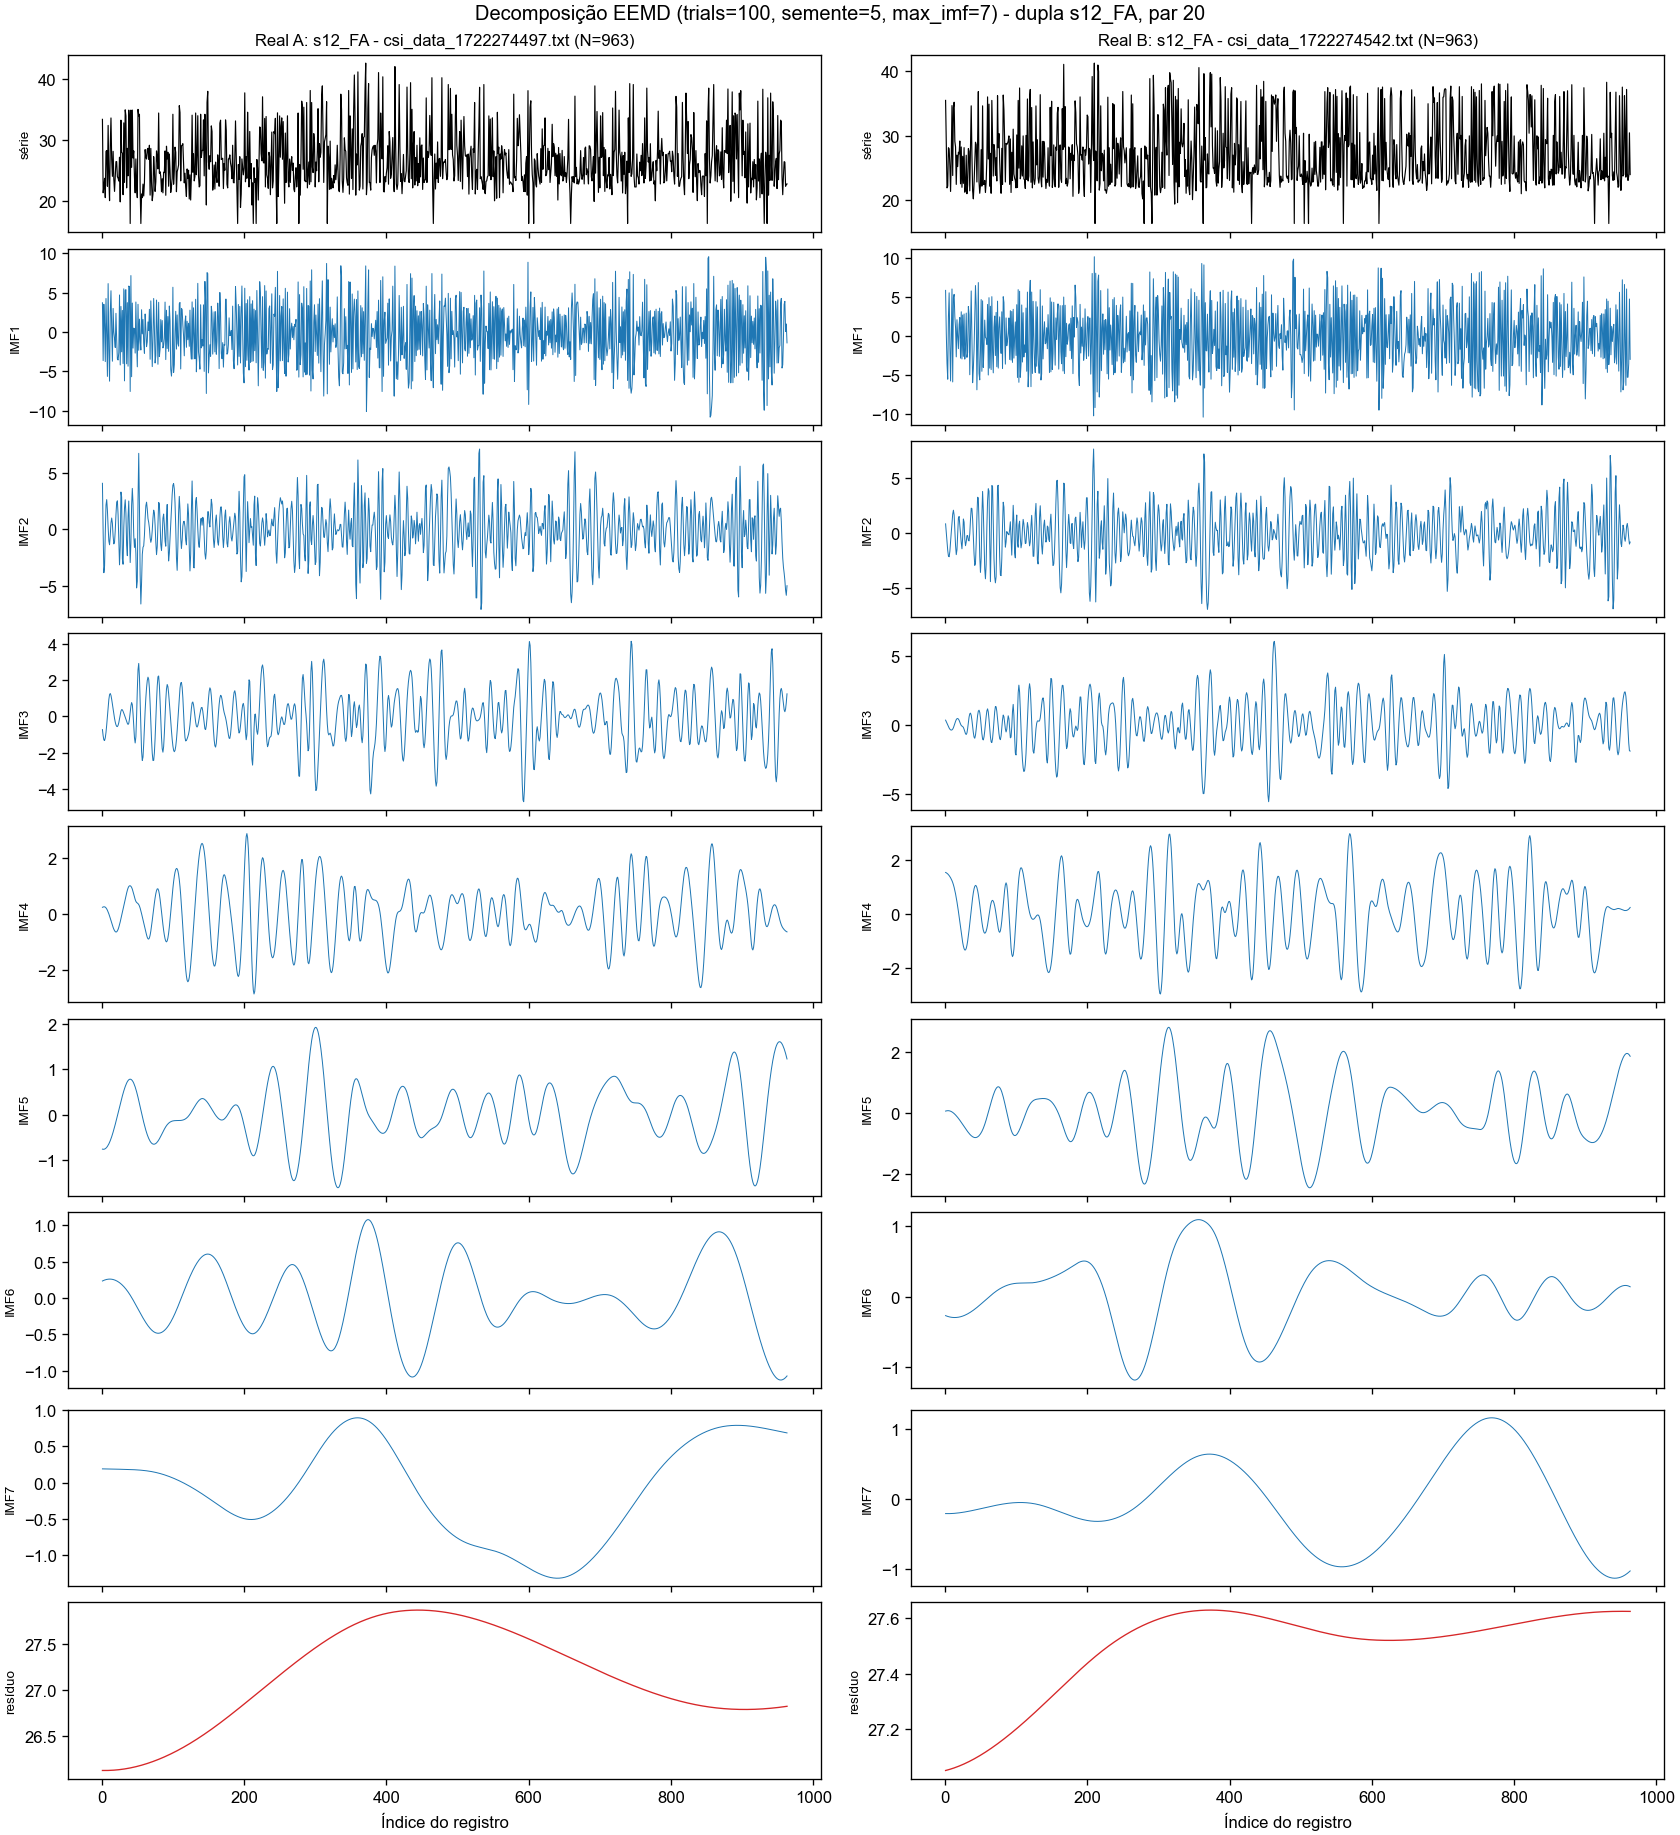
\includegraphics[width=1.00\textwidth,height=19.0cm,keepaspectratio]{Imagens/sec5_decomposicao_s12_FA.png}
    \caption{Decomposição EEMD da dupla s12\_FA (s12, FA): série real do par 20 após o ajuste para N = 963, IMF1 a IMF7 e resíduo. Esquerda: A = Datasets/Activity/FA/s12/csi\_data\_1722274497.txt; direita: B = Datasets/Activity/FA/s12/csi\_data\_1722274542.txt. (arquivo: figuras/sec5\_decomposicao\_s12\_FA.png)}
    \label{fig:sec5_decomposicao_s12_FA}
\end{figure}

\subsection{Comparação entre sinais reais e sintéticos}

As Figuras 12 a 26 mostram, para cada dupla, Real A, Real B e o sinal sintético alinhados verticalmente, com os mesmos limites nos dois eixos dos três gráficos.

\begin{figure}[H]
    \centering
    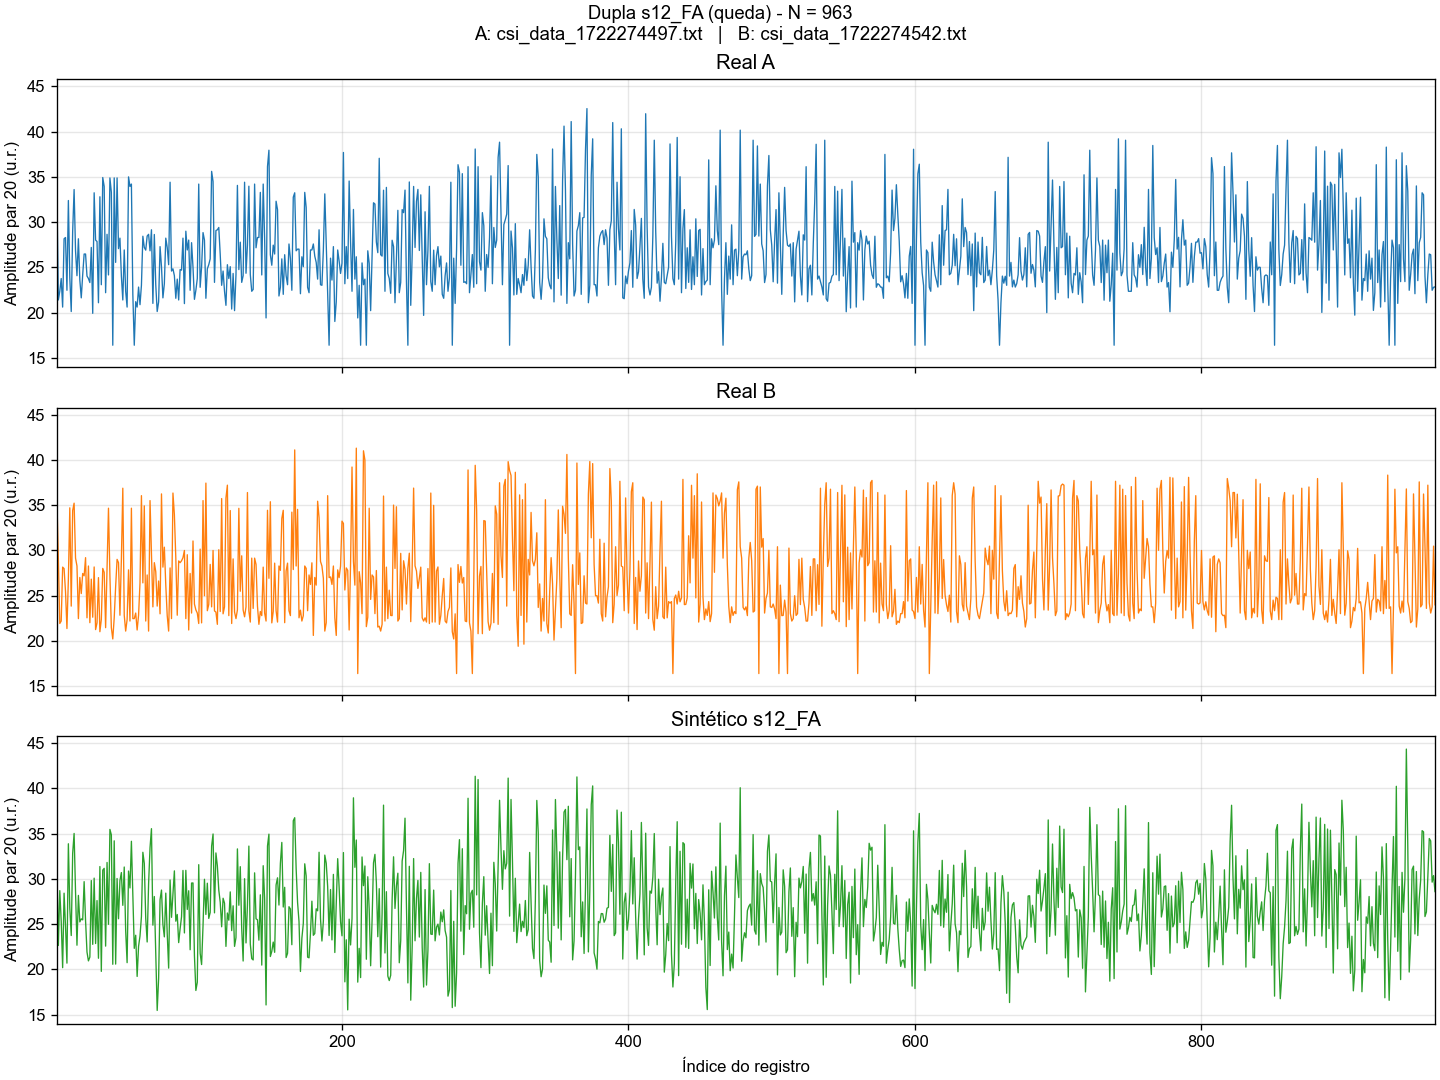
\includegraphics[width=0.79\textwidth,height=19.0cm,keepaspectratio]{Imagens/sec5_comparacao_s12_FA.png}
    \caption{Dupla s12\_FA: Real A (csi\_data\_1722274497.txt), Real B (csi\_data\_1722274542.txt) e Sintético s12\_FA, N = 963. (arquivo: figuras/sec5\_comparacao\_s12\_FA.png)}
    \label{fig:sec5_comparacao_s12_FA}
\end{figure}

\begin{figure}[H]
    \centering
    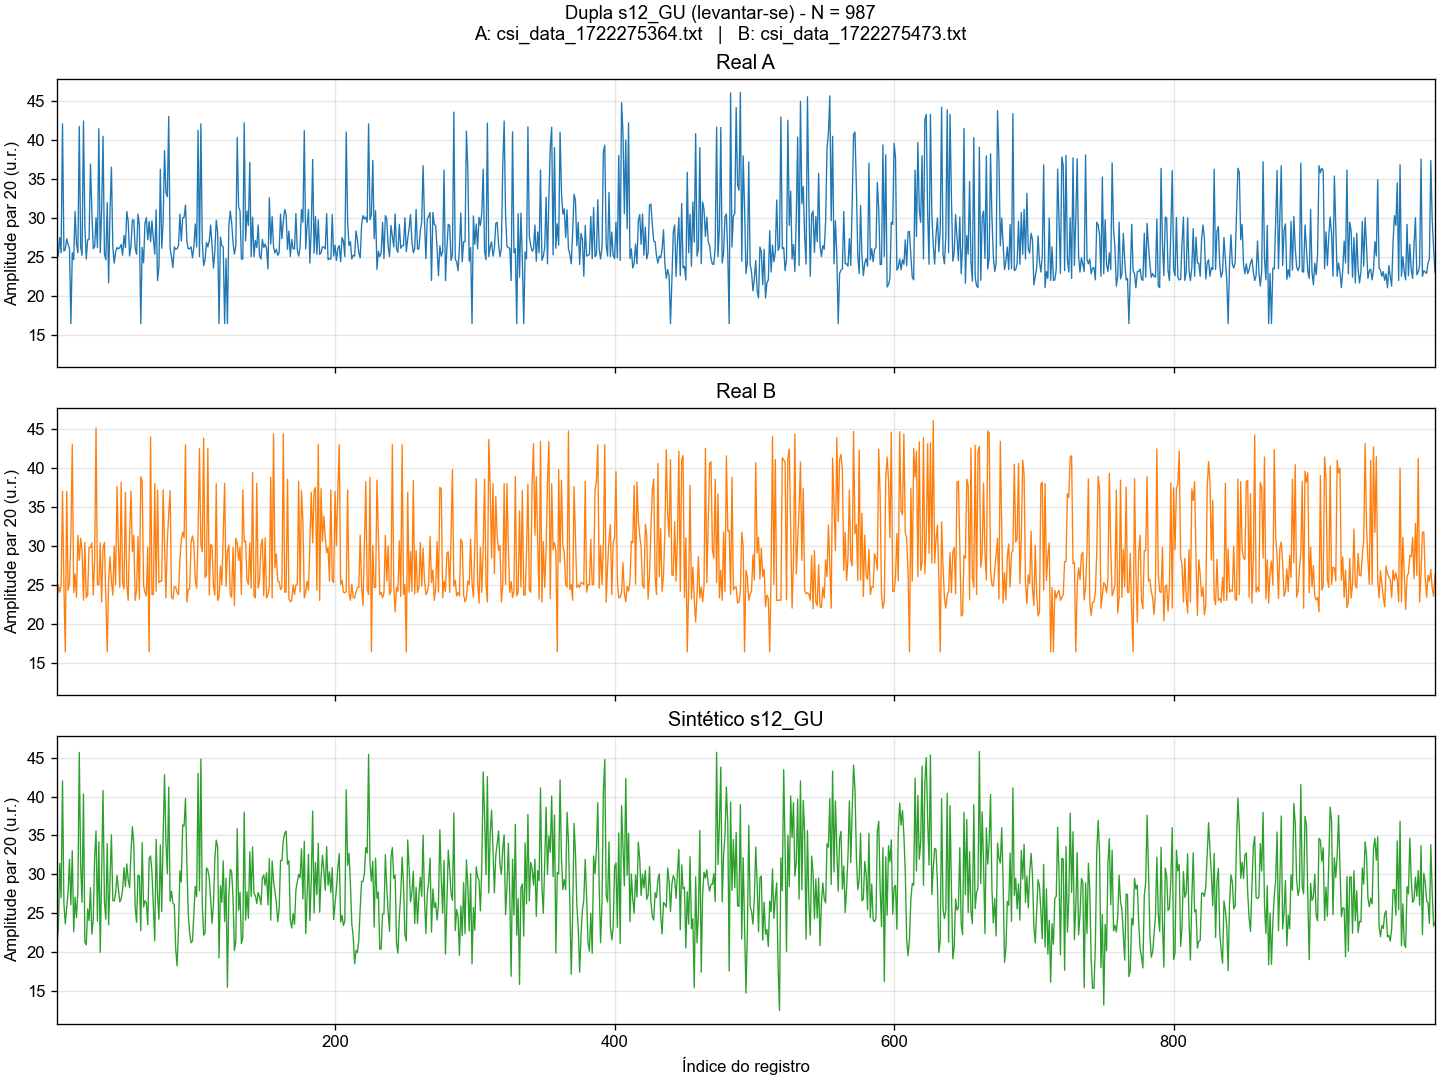
\includegraphics[width=0.79\textwidth,height=19.0cm,keepaspectratio]{Imagens/sec5_comparacao_s12_GU.png}
    \caption{Dupla s12\_GU: Real A (csi\_data\_1722275364.txt), Real B (csi\_data\_1722275473.txt) e Sintético s12\_GU, N = 987. (arquivo: figuras/sec5\_comparacao\_s12\_GU.png)}
    \label{fig:sec5_comparacao_s12_GU}
\end{figure}

\begin{figure}[H]
    \centering
    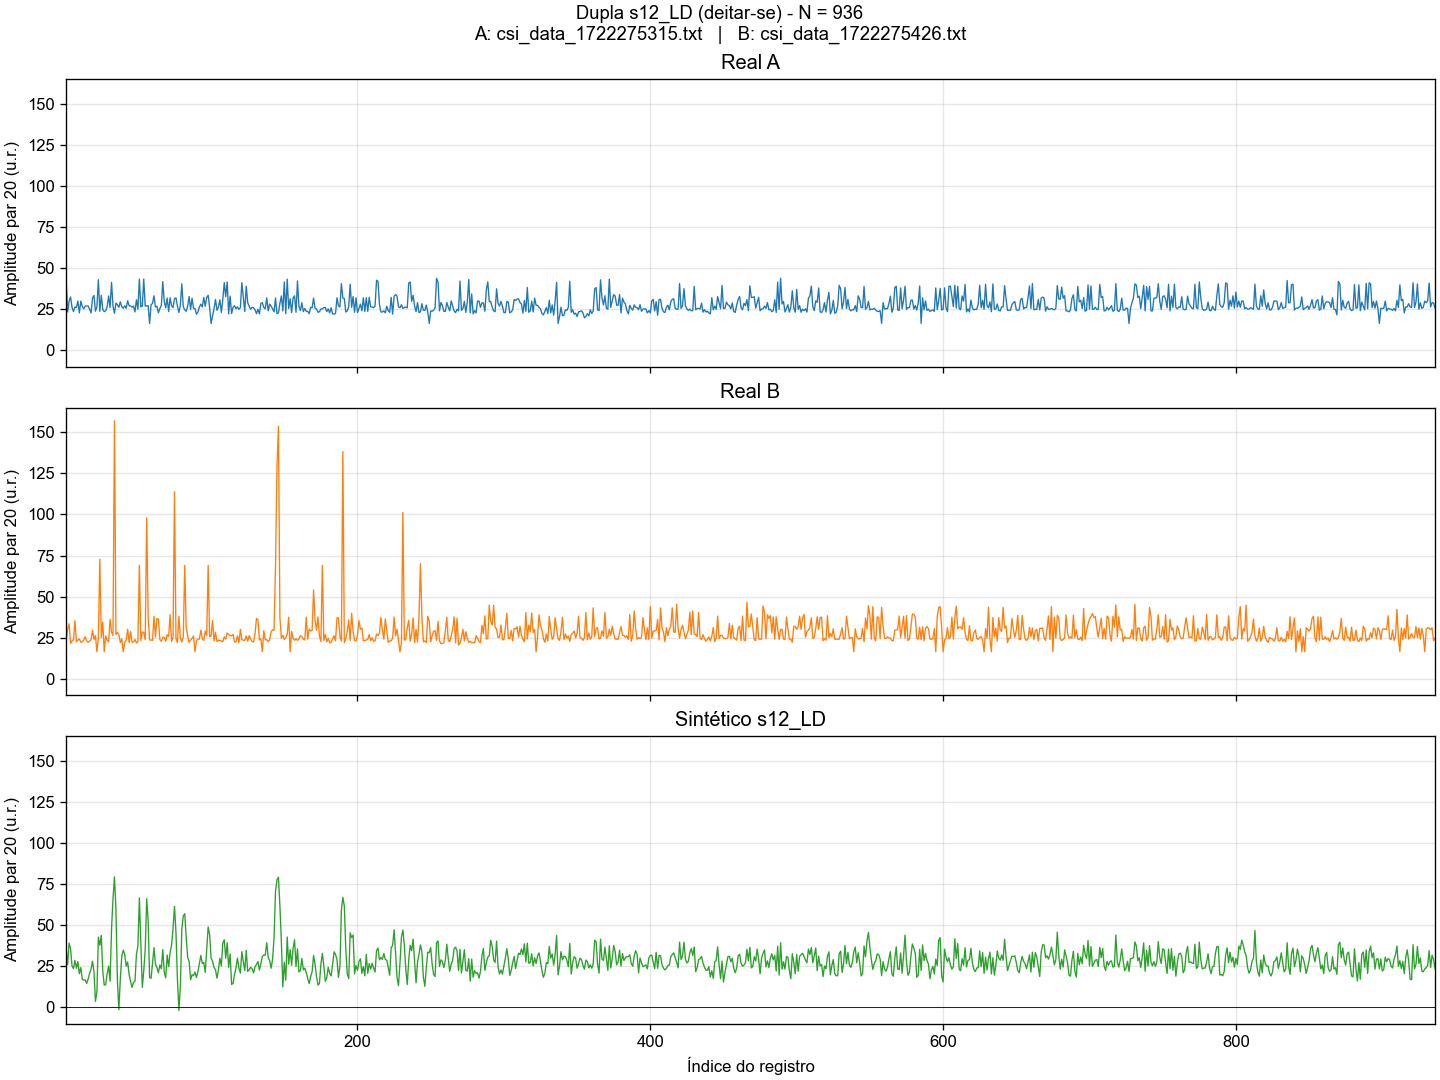
\includegraphics[width=0.79\textwidth,height=19.0cm,keepaspectratio]{Imagens/sec5_comparacao_s12_LD.png}
    \caption{Dupla s12\_LD: Real A (csi\_data\_1722275315.txt), Real B (csi\_data\_1722275426.txt) e Sintético s12\_LD, N = 936. (arquivo: figuras/sec5\_comparacao\_s12\_LD.png)}
    \label{fig:sec5_comparacao_s12_LD}
\end{figure}

\begin{figure}[H]
    \centering
    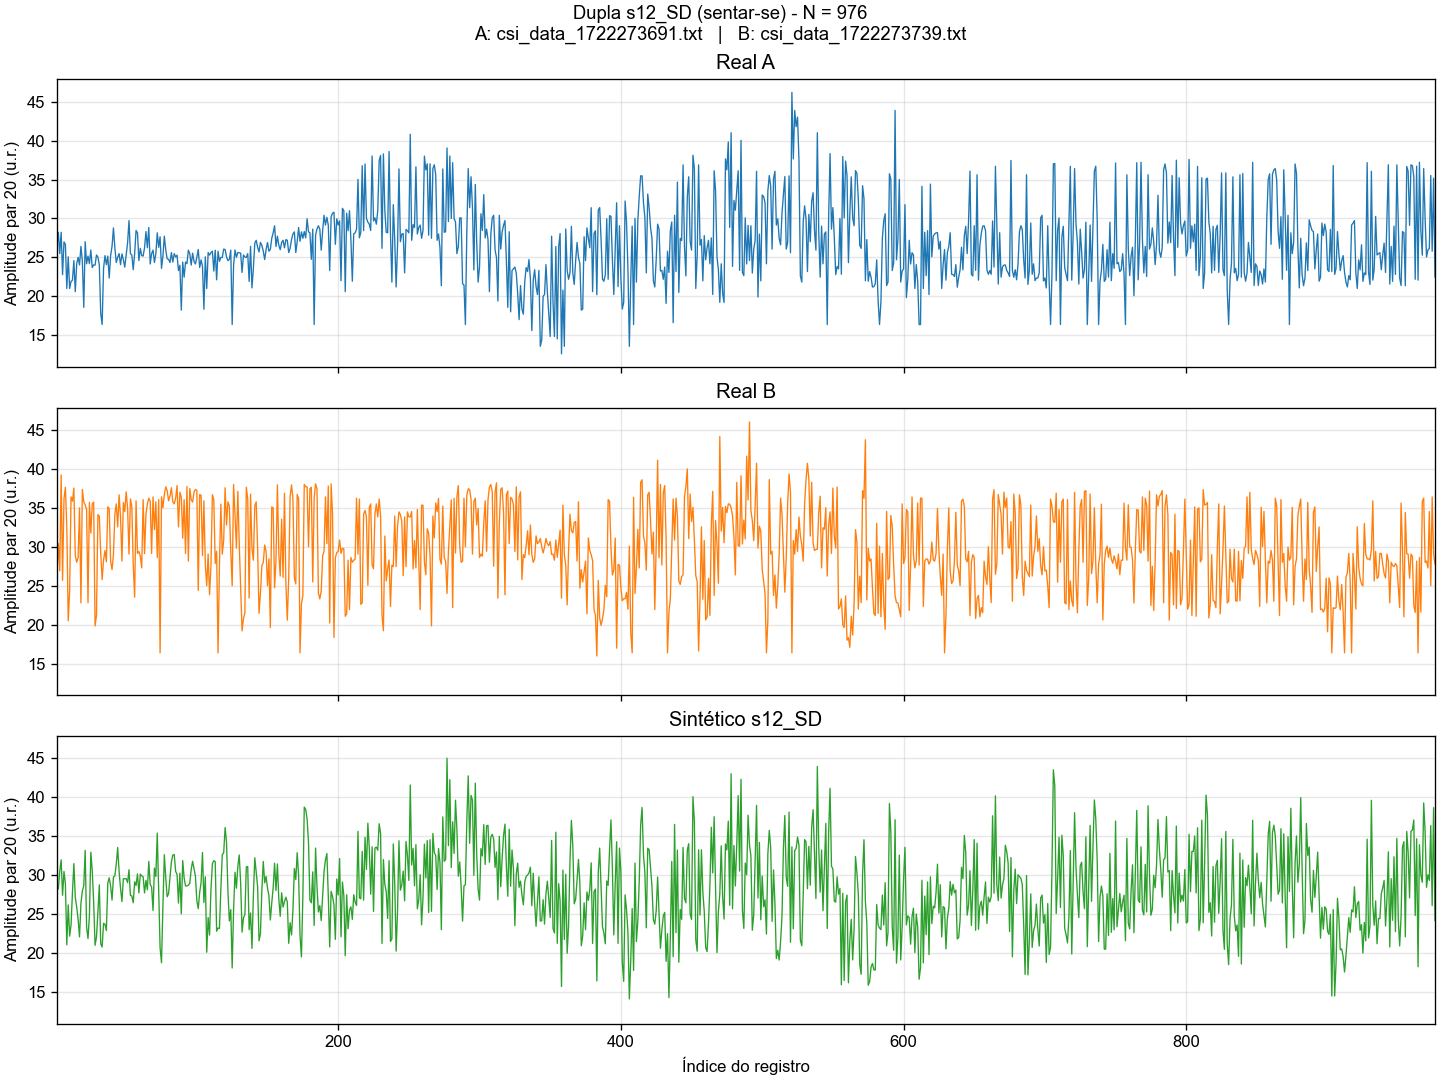
\includegraphics[width=0.79\textwidth,height=19.0cm,keepaspectratio]{Imagens/sec5_comparacao_s12_SD.png}
    \caption{Dupla s12\_SD: Real A (csi\_data\_1722273691.txt), Real B (csi\_data\_1722273739.txt) e Sintético s12\_SD, N = 976. (arquivo: figuras/sec5\_comparacao\_s12\_SD.png)}
    \label{fig:sec5_comparacao_s12_SD}
\end{figure}

\begin{figure}[H]
    \centering
    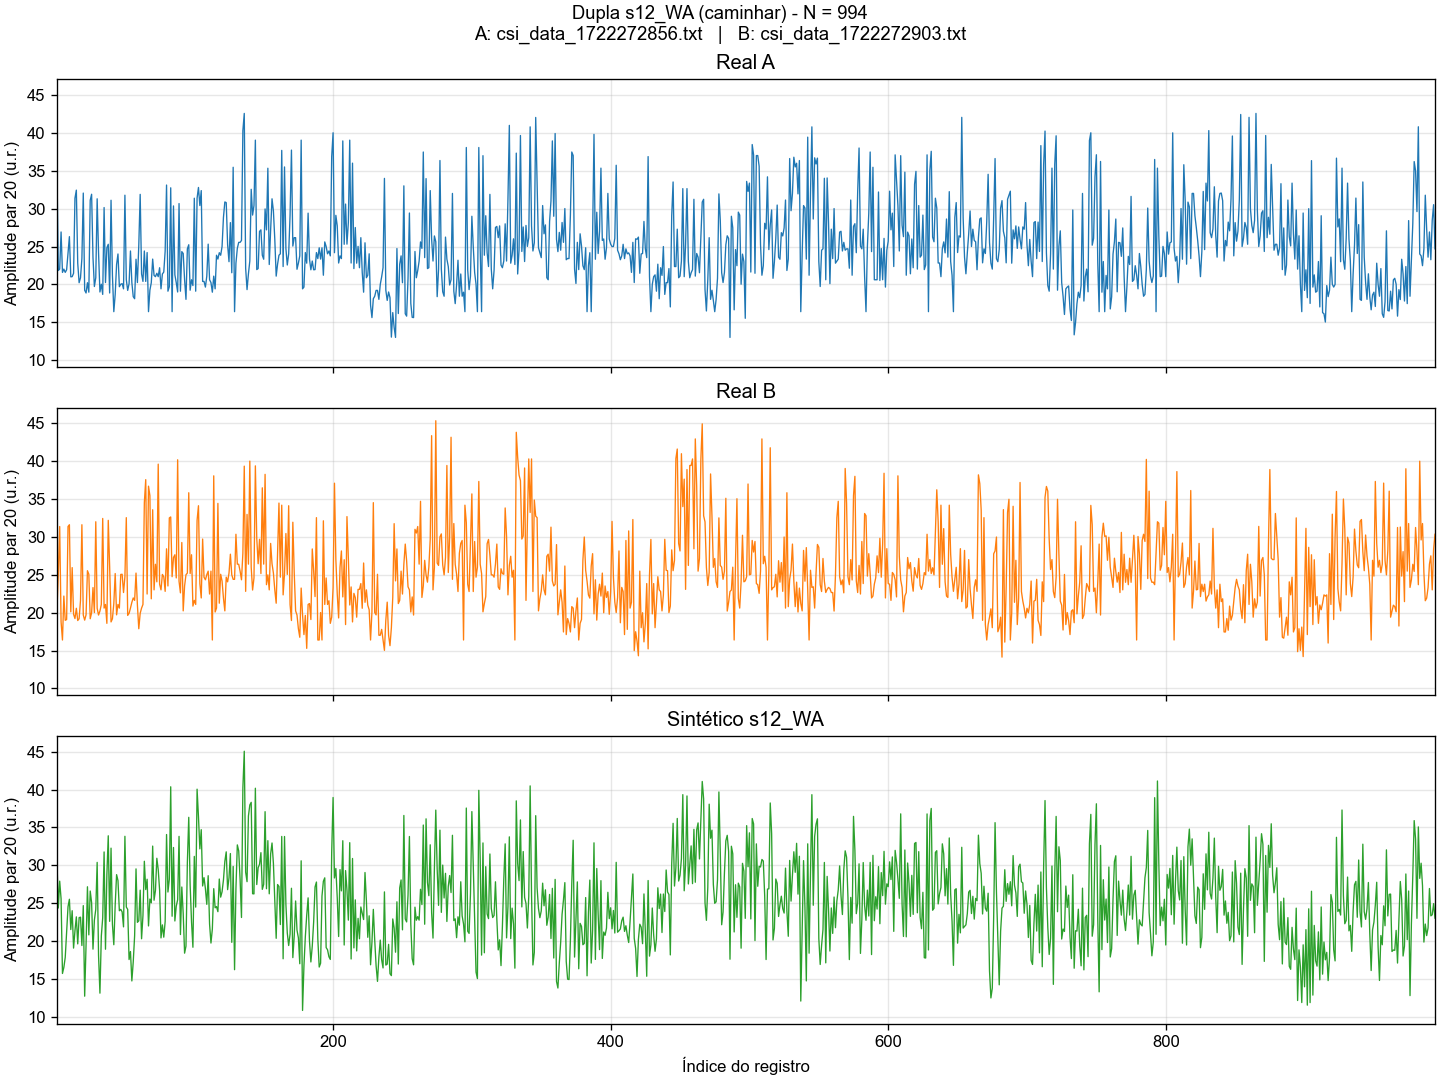
\includegraphics[width=0.79\textwidth,height=19.0cm,keepaspectratio]{Imagens/sec5_comparacao_s12_WA.png}
    \caption{Dupla s12\_WA: Real A (csi\_data\_1722272856.txt), Real B (csi\_data\_1722272903.txt) e Sintético s12\_WA, N = 994. (arquivo: figuras/sec5\_comparacao\_s12\_WA.png)}
    \label{fig:sec5_comparacao_s12_WA}
\end{figure}

\begin{figure}[H]
    \centering
    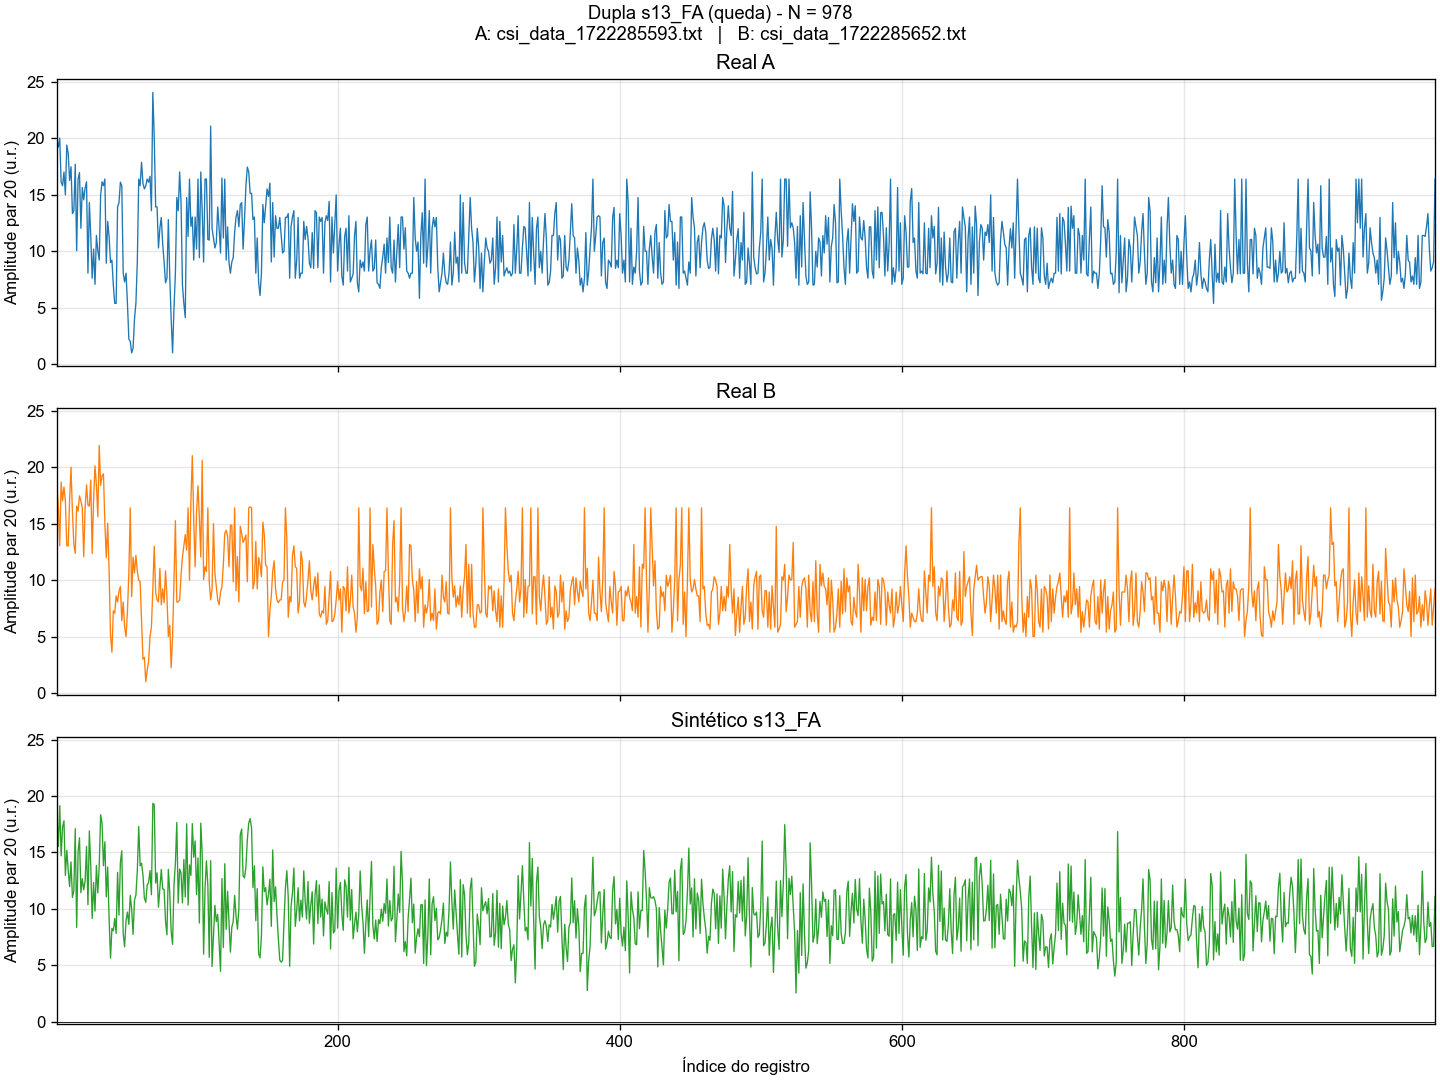
\includegraphics[width=0.79\textwidth,height=19.0cm,keepaspectratio]{Imagens/sec5_comparacao_s13_FA.png}
    \caption{Dupla s13\_FA: Real A (csi\_data\_1722285593.txt), Real B (csi\_data\_1722285652.txt) e Sintético s13\_FA, N = 978. (arquivo: figuras/sec5\_comparacao\_s13\_FA.png)}
    \label{fig:sec5_comparacao_s13_FA}
\end{figure}

\begin{figure}[H]
    \centering
    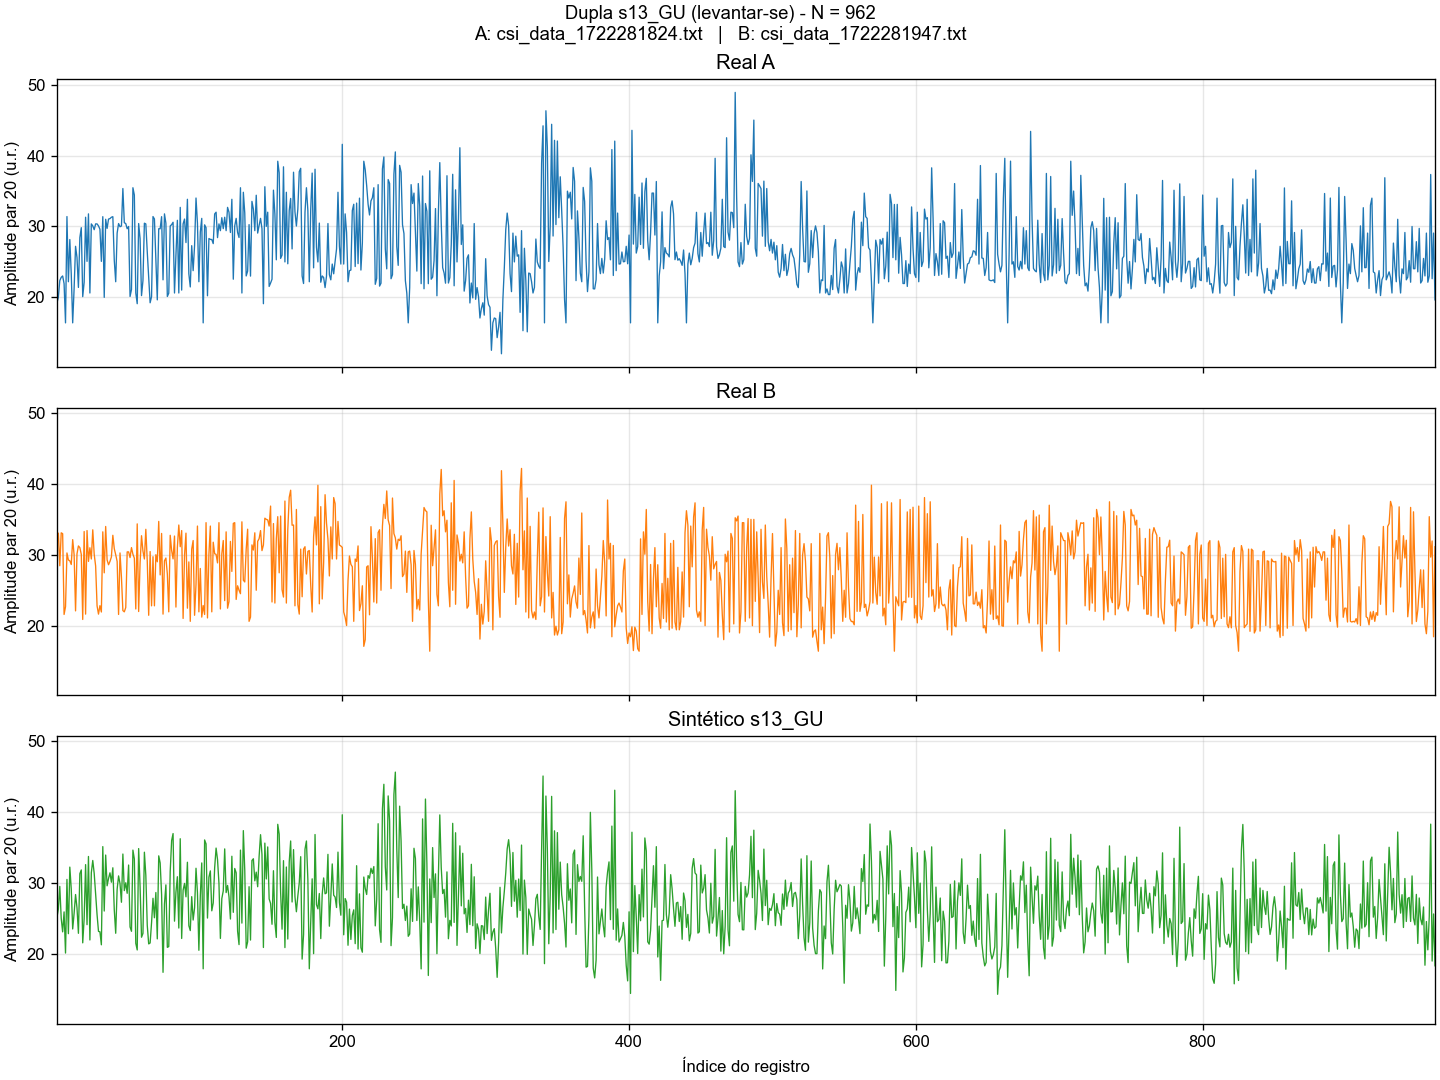
\includegraphics[width=0.79\textwidth,height=19.0cm,keepaspectratio]{Imagens/sec5_comparacao_s13_GU.png}
    \caption{Dupla s13\_GU: Real A (csi\_data\_1722281824.txt), Real B (csi\_data\_1722281947.txt) e Sintético s13\_GU, N = 962. (arquivo: figuras/sec5\_comparacao\_s13\_GU.png)}
    \label{fig:sec5_comparacao_s13_GU}
\end{figure}

\begin{figure}[H]
    \centering
    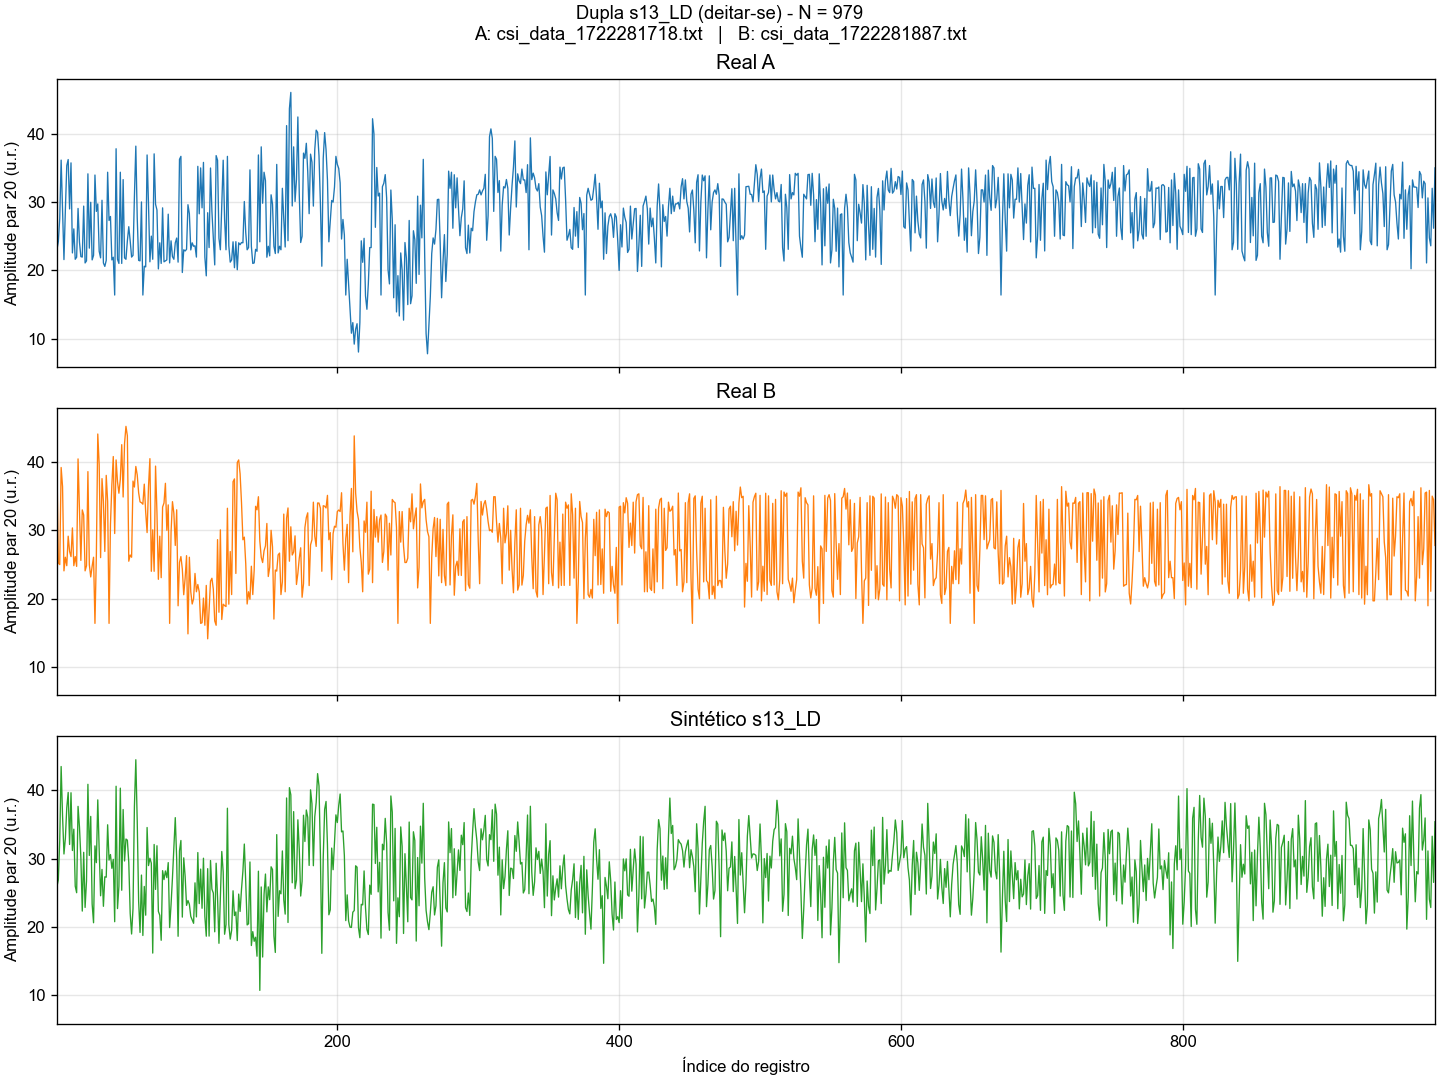
\includegraphics[width=0.79\textwidth,height=19.0cm,keepaspectratio]{Imagens/sec5_comparacao_s13_LD.png}
    \caption{Dupla s13\_LD: Real A (csi\_data\_1722281718.txt), Real B (csi\_data\_1722281887.txt) e Sintético s13\_LD, N = 979. (arquivo: figuras/sec5\_comparacao\_s13\_LD.png)}
    \label{fig:sec5_comparacao_s13_LD}
\end{figure}

\begin{figure}[H]
    \centering
    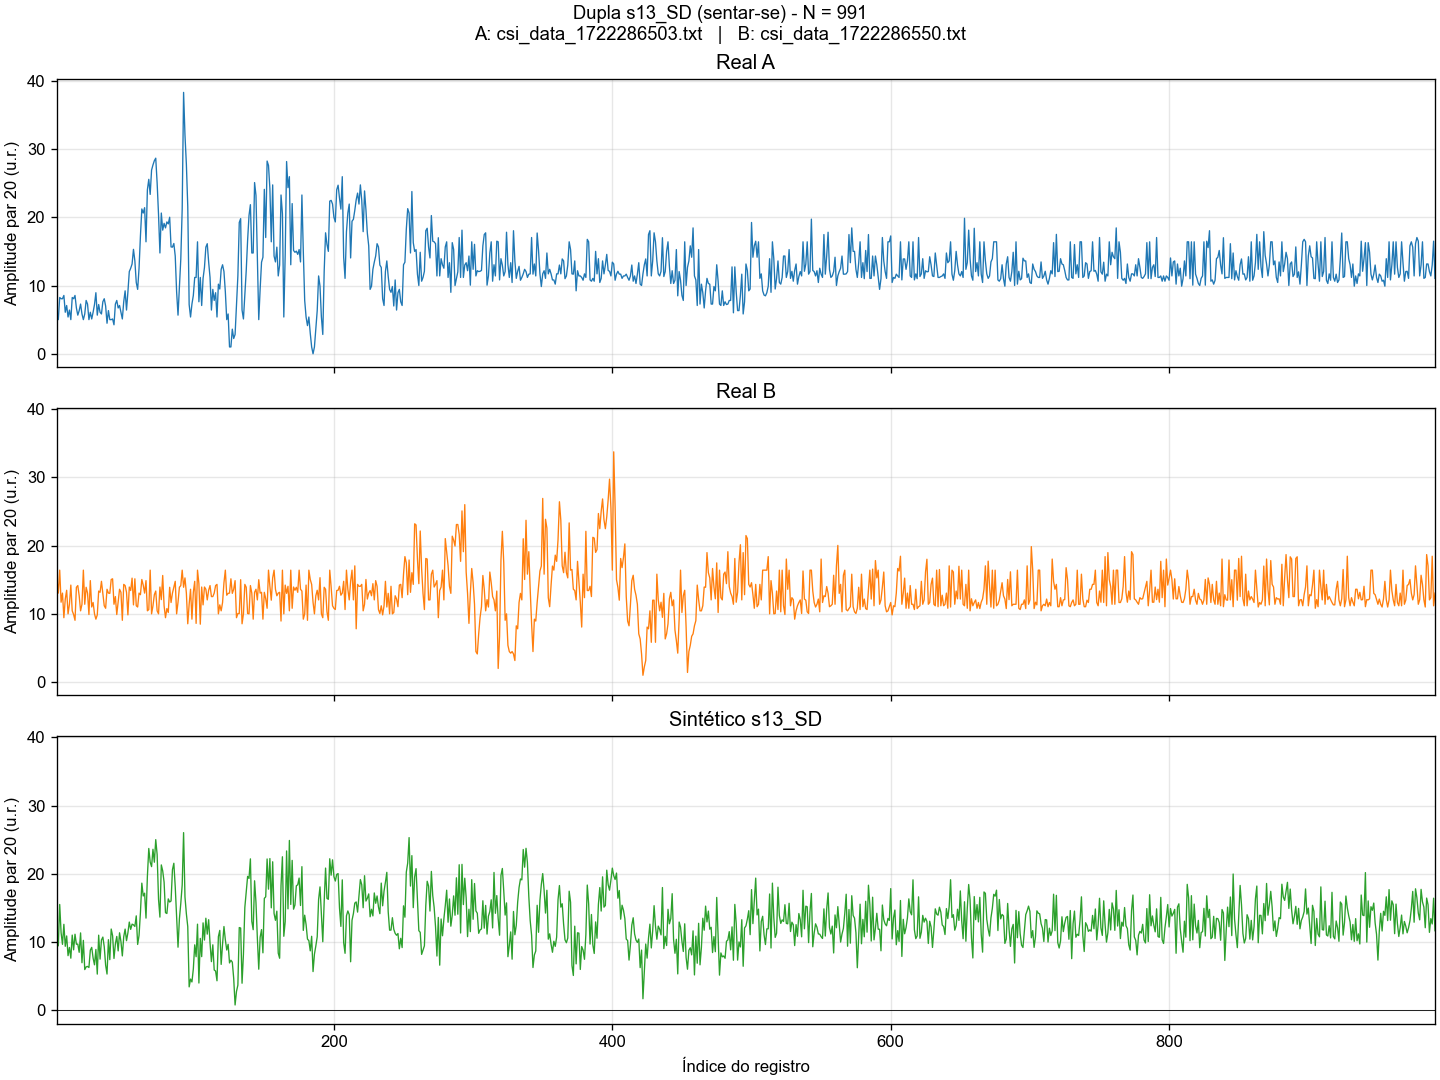
\includegraphics[width=0.79\textwidth,height=19.0cm,keepaspectratio]{Imagens/sec5_comparacao_s13_SD.png}
    \caption{Dupla s13\_SD: Real A (csi\_data\_1722286503.txt), Real B (csi\_data\_1722286550.txt) e Sintético s13\_SD, N = 991. (arquivo: figuras/sec5\_comparacao\_s13\_SD.png)}
    \label{fig:sec5_comparacao_s13_SD}
\end{figure}

\begin{figure}[H]
    \centering
    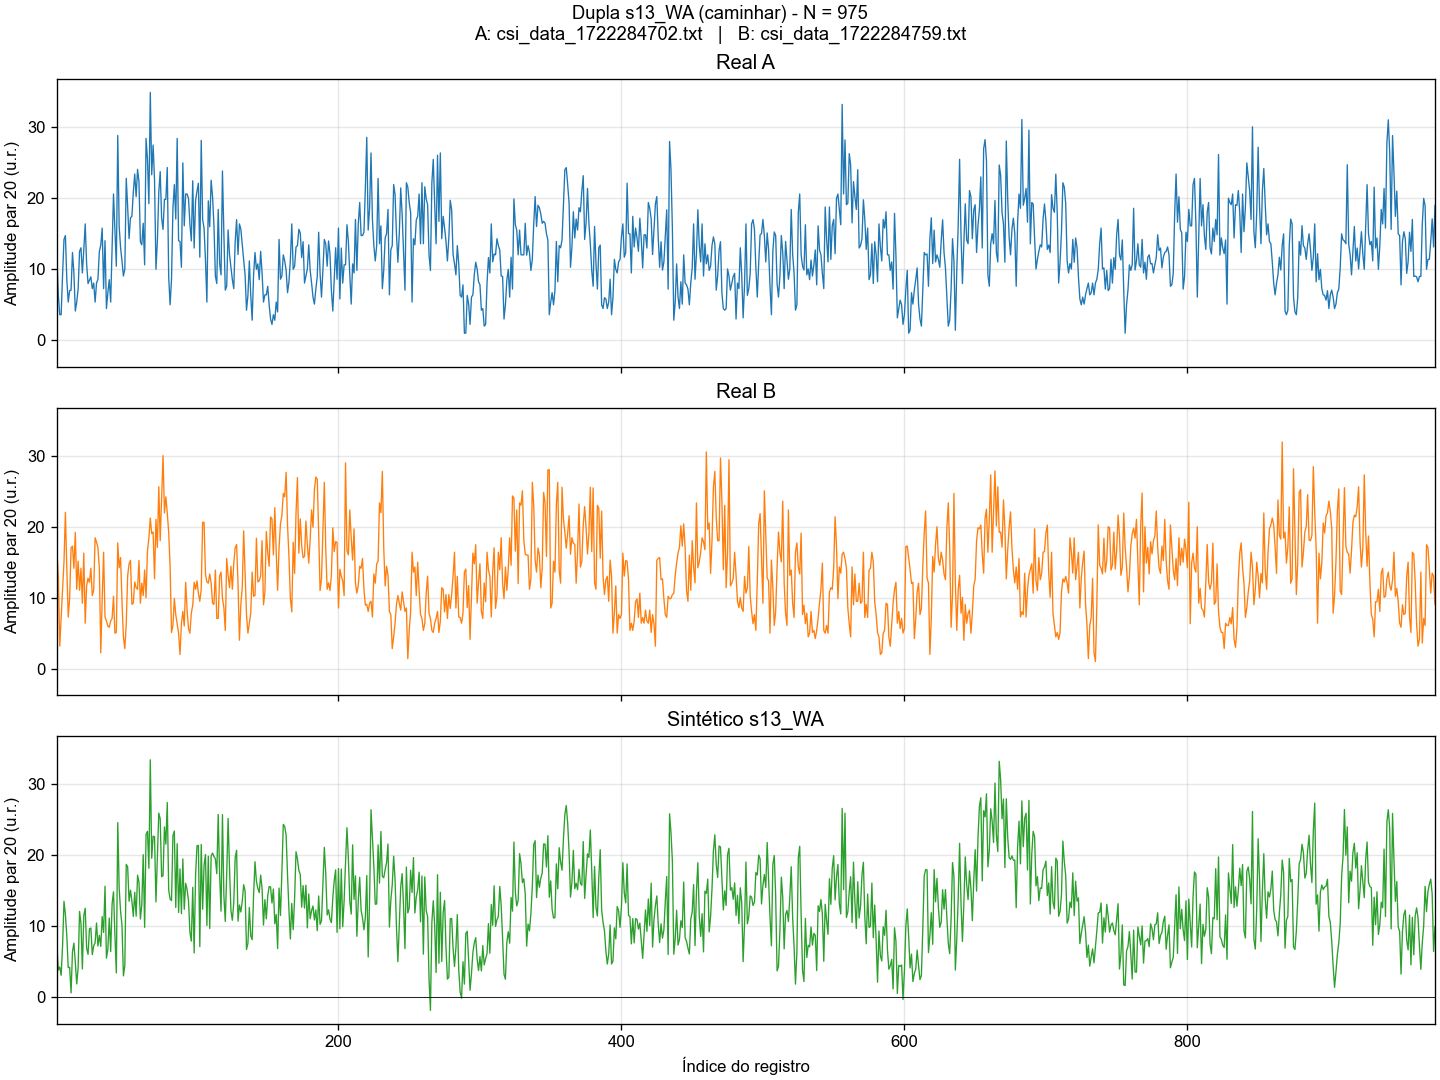
\includegraphics[width=0.79\textwidth,height=19.0cm,keepaspectratio]{Imagens/sec5_comparacao_s13_WA.png}
    \caption{Dupla s13\_WA: Real A (csi\_data\_1722284702.txt), Real B (csi\_data\_1722284759.txt) e Sintético s13\_WA, N = 975. (arquivo: figuras/sec5\_comparacao\_s13\_WA.png)}
    \label{fig:sec5_comparacao_s13_WA}
\end{figure}

\begin{figure}[H]
    \centering
    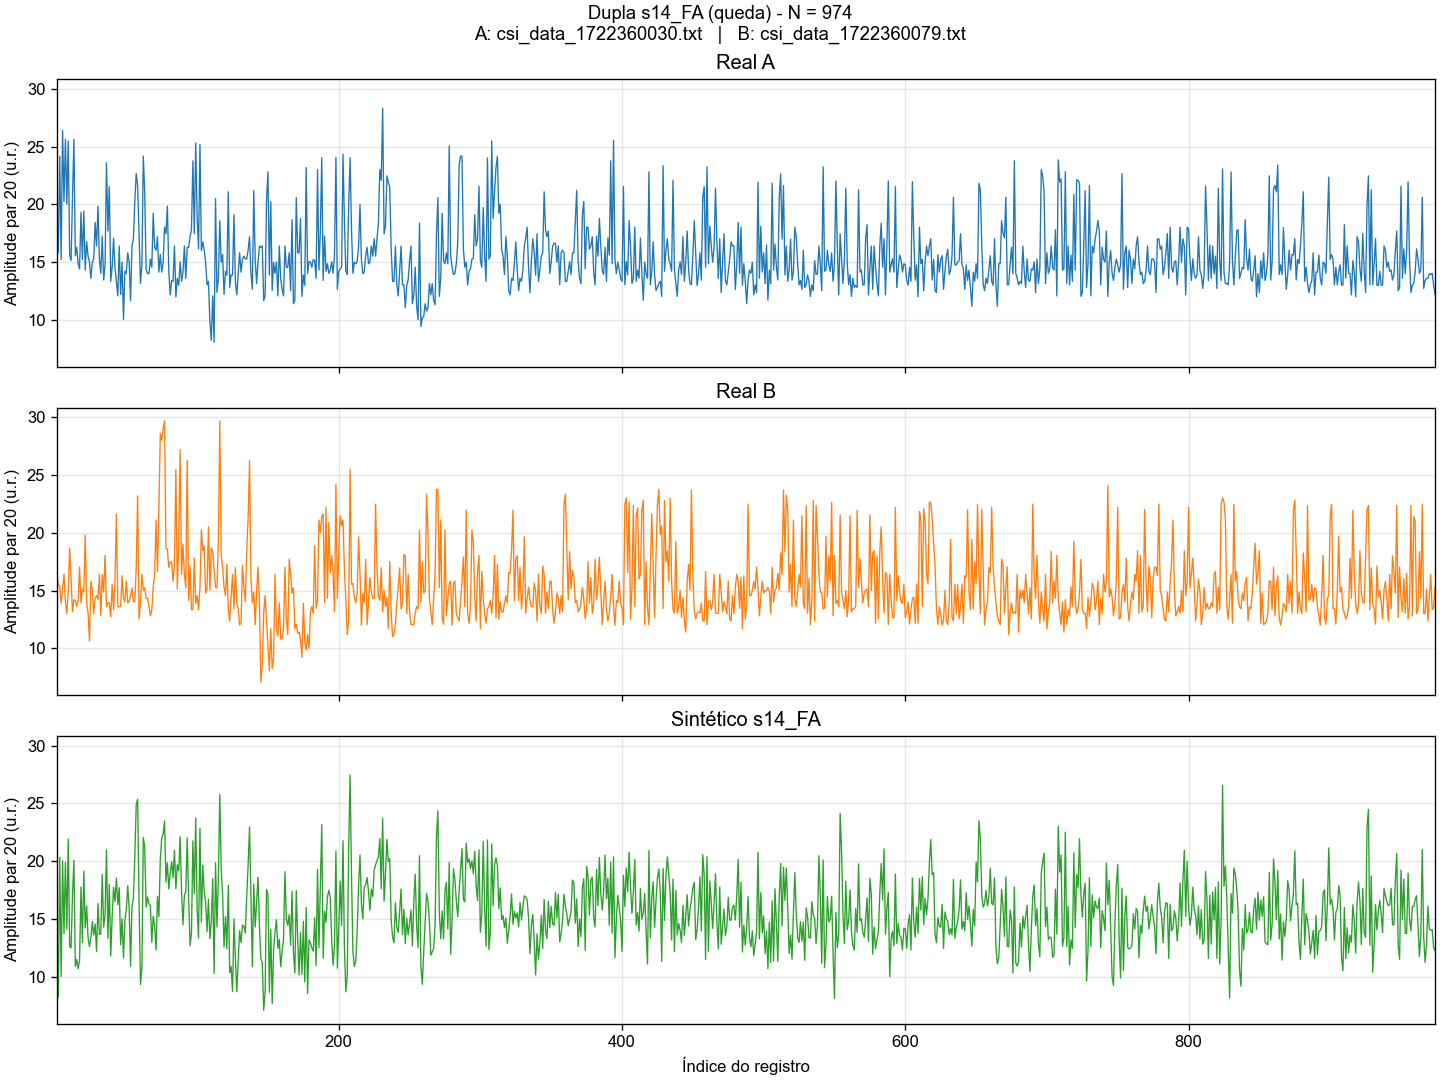
\includegraphics[width=0.79\textwidth,height=19.0cm,keepaspectratio]{Imagens/sec5_comparacao_s14_FA.png}
    \caption{Dupla s14\_FA: Real A (csi\_data\_1722360030.txt), Real B (csi\_data\_1722360079.txt) e Sintético s14\_FA, N = 974. (arquivo: figuras/sec5\_comparacao\_s14\_FA.png)}
    \label{fig:sec5_comparacao_s14_FA}
\end{figure}

\begin{figure}[H]
    \centering
    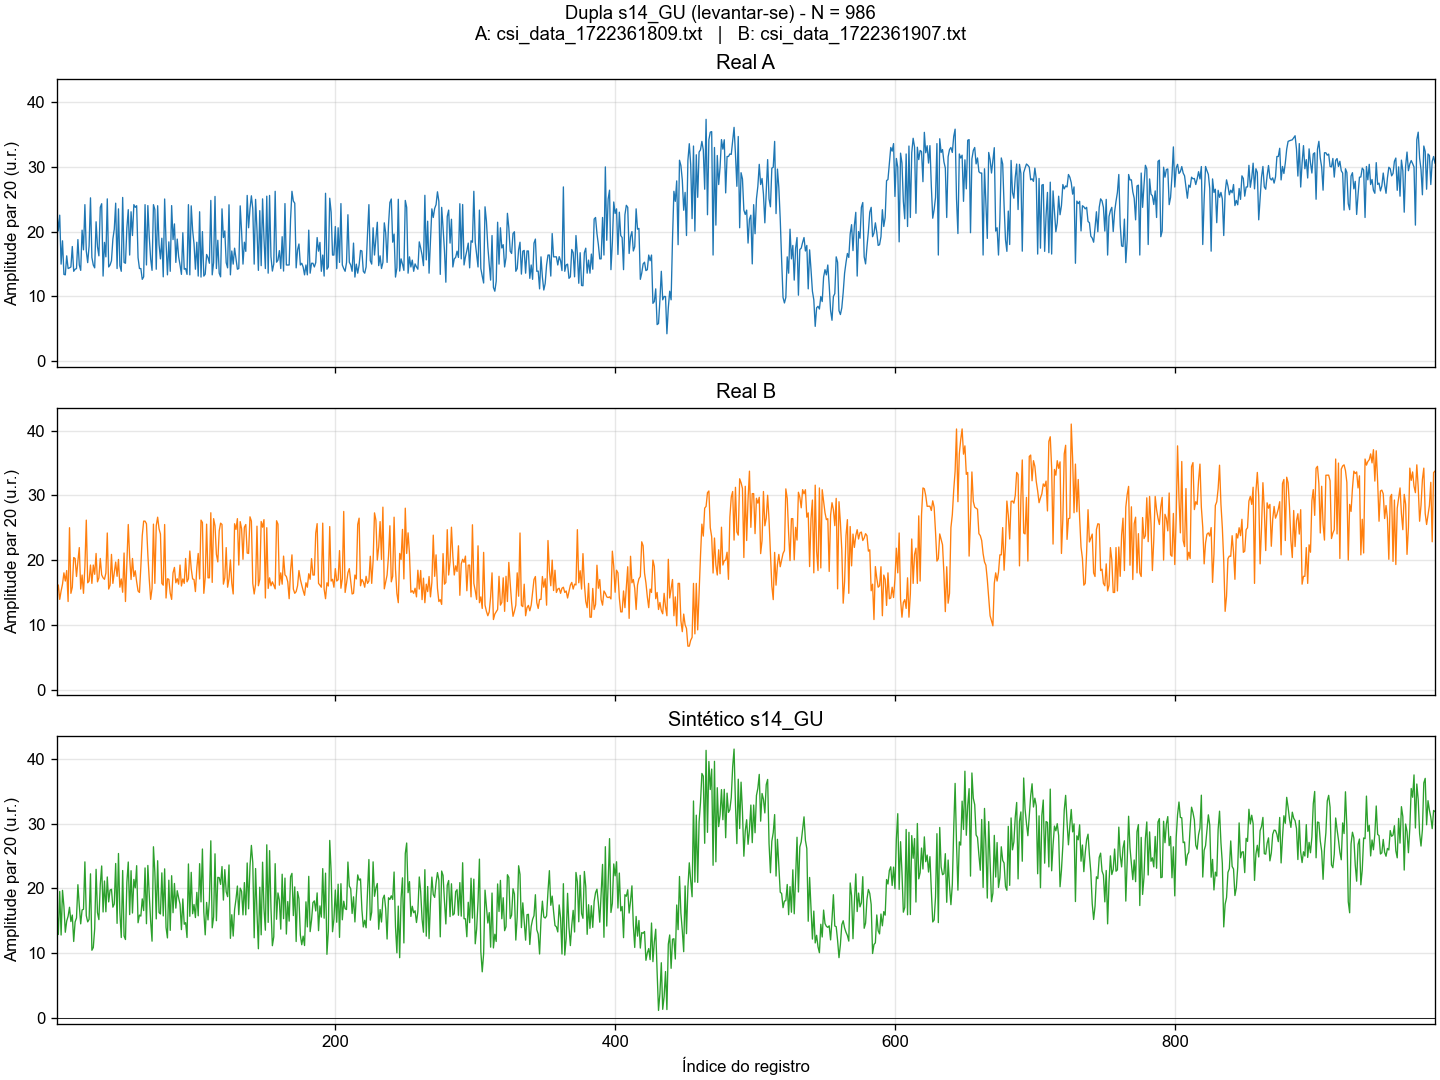
\includegraphics[width=0.79\textwidth,height=19.0cm,keepaspectratio]{Imagens/sec5_comparacao_s14_GU.png}
    \caption{Dupla s14\_GU: Real A (csi\_data\_1722361809.txt), Real B (csi\_data\_1722361907.txt) e Sintético s14\_GU, N = 986. (arquivo: figuras/sec5\_comparacao\_s14\_GU.png)}
    \label{fig:sec5_comparacao_s14_GU}
\end{figure}

\begin{figure}[H]
    \centering
    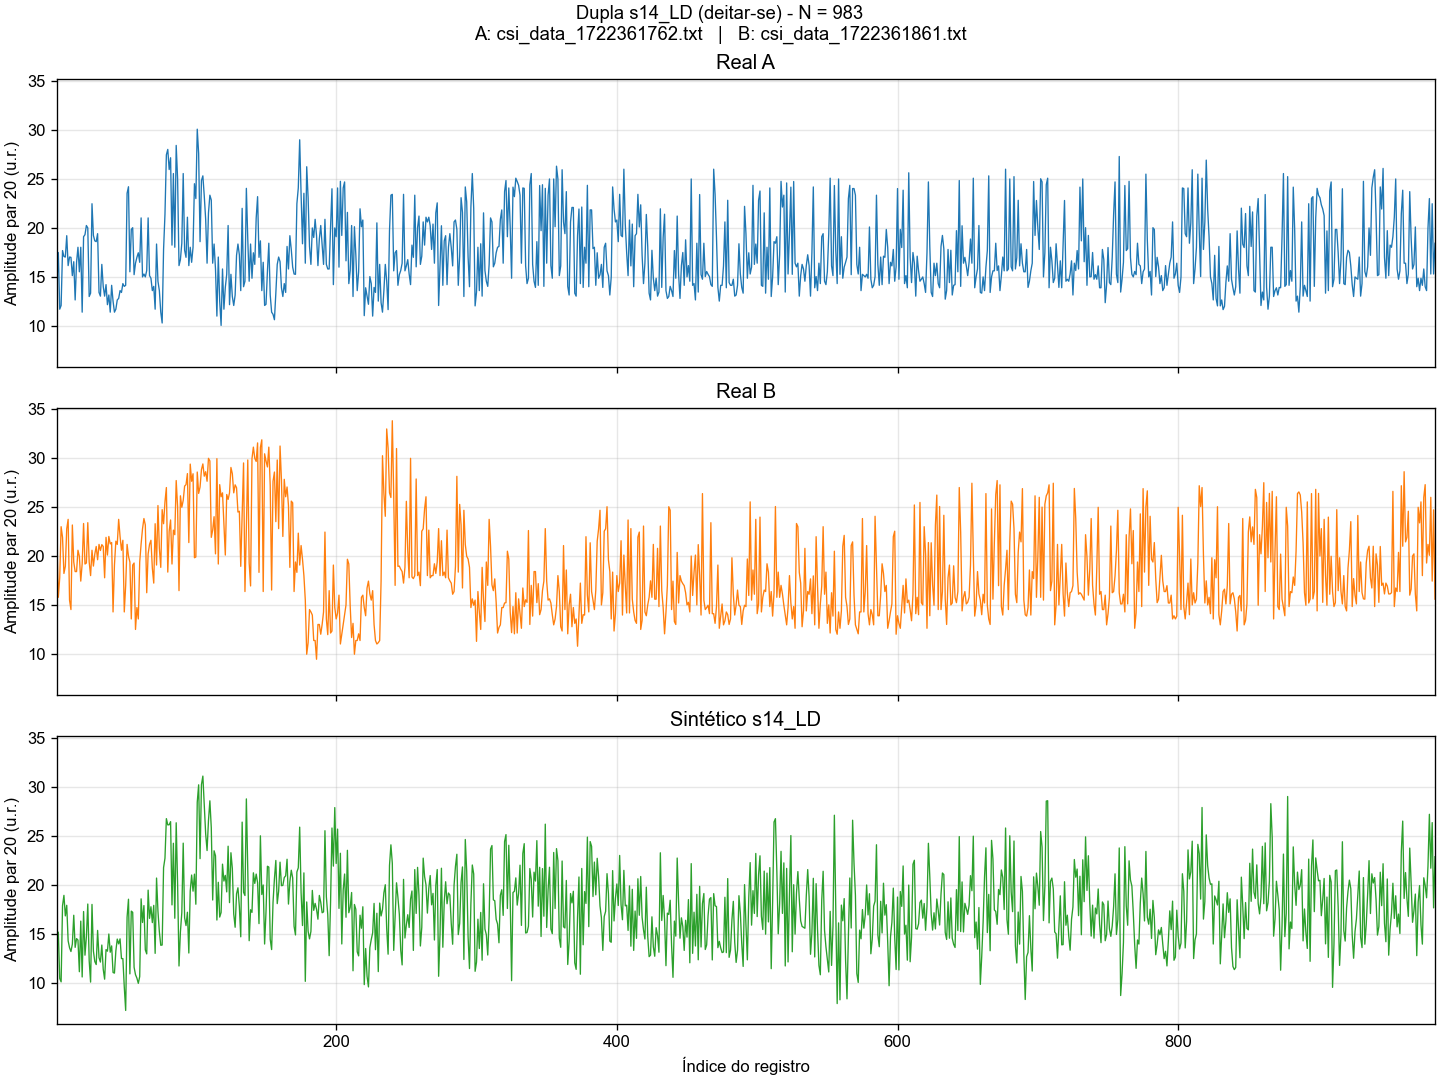
\includegraphics[width=0.79\textwidth,height=19.0cm,keepaspectratio]{Imagens/sec5_comparacao_s14_LD.png}
    \caption{Dupla s14\_LD: Real A (csi\_data\_1722361762.txt), Real B (csi\_data\_1722361861.txt) e Sintético s14\_LD, N = 983. (arquivo: figuras/sec5\_comparacao\_s14\_LD.png)}
    \label{fig:sec5_comparacao_s14_LD}
\end{figure}

\begin{figure}[H]
    \centering
    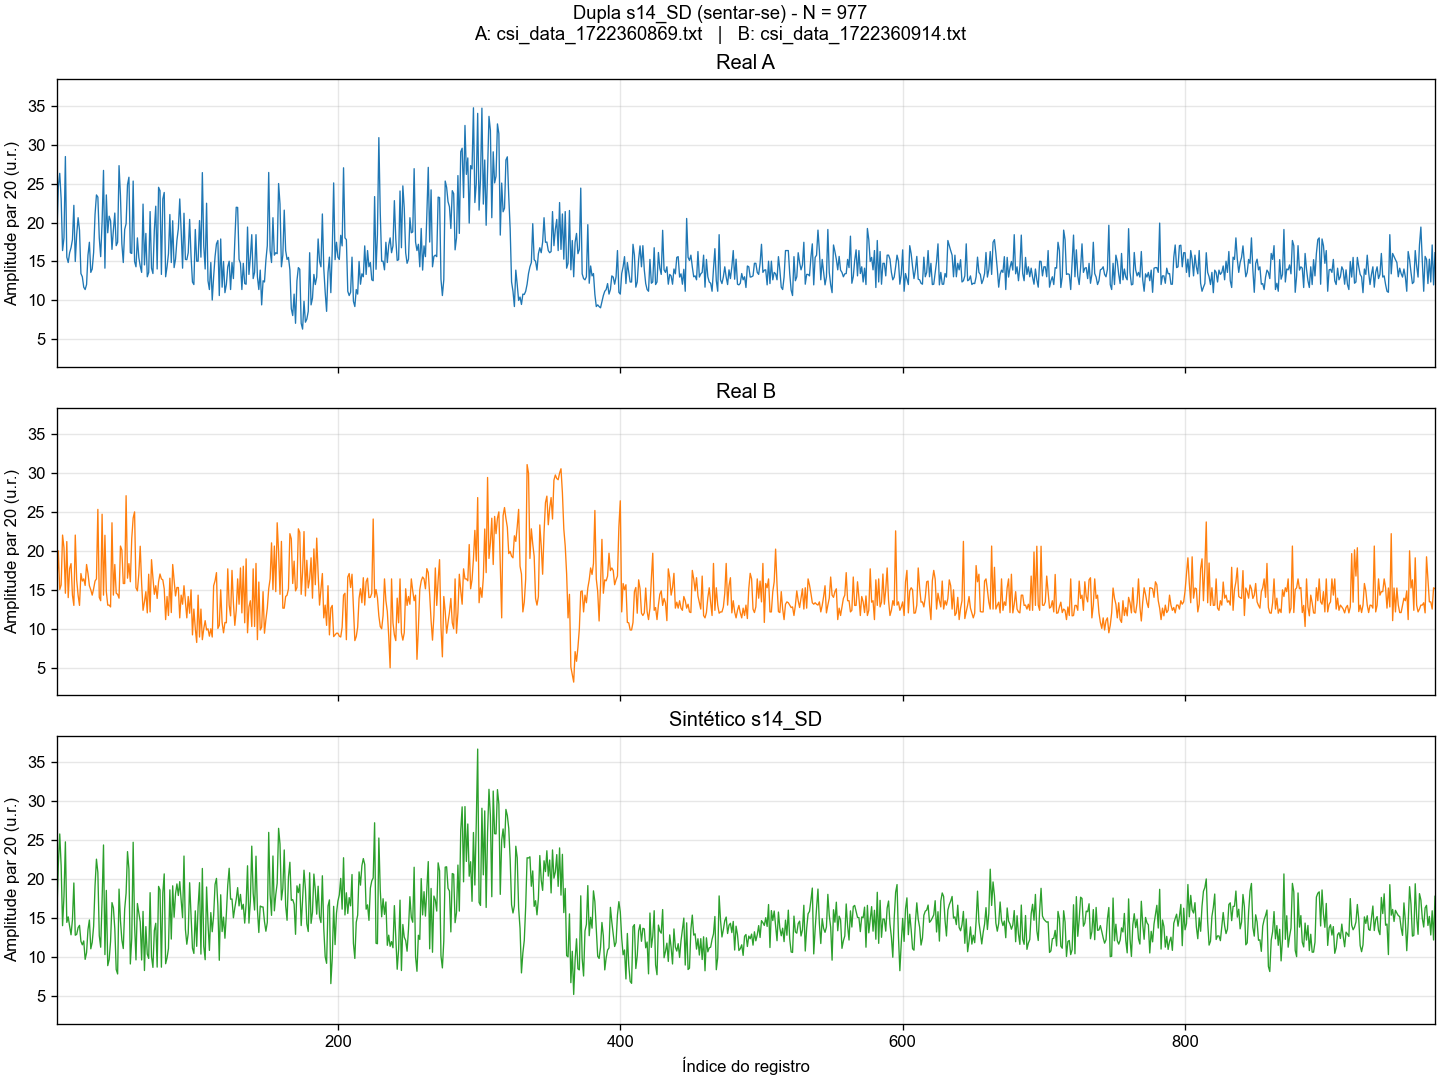
\includegraphics[width=0.79\textwidth,height=19.0cm,keepaspectratio]{Imagens/sec5_comparacao_s14_SD.png}
    \caption{Dupla s14\_SD: Real A (csi\_data\_1722360869.txt), Real B (csi\_data\_1722360914.txt) e Sintético s14\_SD, N = 977. (arquivo: figuras/sec5\_comparacao\_s14\_SD.png)}
    \label{fig:sec5_comparacao_s14_SD}
\end{figure}

\begin{figure}[H]
    \centering
    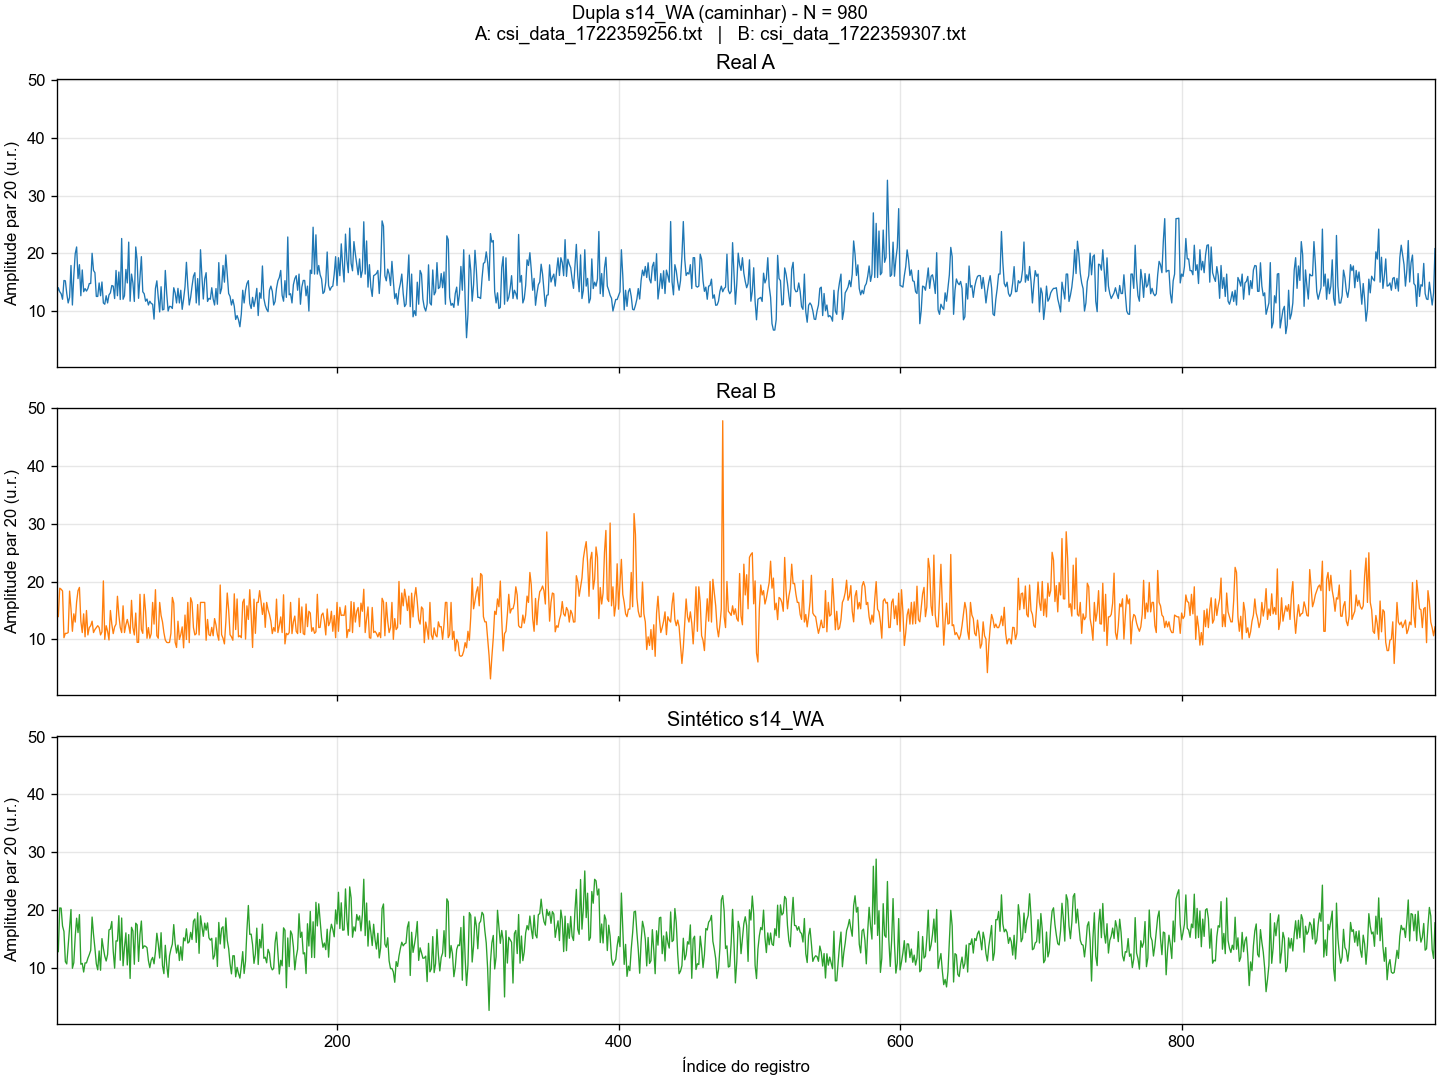
\includegraphics[width=0.79\textwidth,height=19.0cm,keepaspectratio]{Imagens/sec5_comparacao_s14_WA.png}
    \caption{Dupla s14\_WA: Real A (csi\_data\_1722359256.txt), Real B (csi\_data\_1722359307.txt) e Sintético s14\_WA, N = 980. (arquivo: figuras/sec5\_comparacao\_s14\_WA.png)}
    \label{fig:sec5_comparacao_s14_WA}
\end{figure}

\subsection{Características dos sinais comparados}

As cinco características foram recalculadas para real\_A, real\_B e sintético usando os mesmos N valores (45 linhas em \textbf{caracteristicas\_emd.csv}; tabela completa no Anexo, Tabela A2). Para cada característica, a tabela abaixo conta em quantas das 15 duplas o valor do sintético ficou entre os valores de A e B, acima ou abaixo, e o afastamento relativo médio em relação à média de A e B.

{\footnotesize
\begin{longtable}{|>{\centering\arraybackslash}p{3.24cm}|>{\centering\arraybackslash}p{1.62cm}|>{\centering\arraybackslash}p{1.30cm}|>{\centering\arraybackslash}p{1.30cm}|>{\centering\arraybackslash}p{2.60cm}|>{\centering\arraybackslash}p{3.24cm}|}
\caption{Posição das características do sinal sintético em relação a A e B (15 duplas).}\\
\hline
\textbf{Característica} & \textbf{Entre A e B} & \textbf{Acima} & \textbf{Abaixo} & \textbf{Afastamento médio (\%)} & \textbf{Maior afastamento} \\ \hline
\endfirsthead
\hline
\textbf{Característica} & \textbf{Entre A e B} & \textbf{Acima} & \textbf{Abaixo} & \textbf{Afastamento médio (\%)} & \textbf{Maior afastamento} \\ \hline
\endhead
média & 14 & 1 & 0 & 0,6 & s14\_LD (2,4\%) \\ \hline
mediana & 5 & 9 & 1 & 2,7 & s12\_LD (7,0\%) \\ \hline
desvio padrão & 10 & 2 & 3 & 3,4 & s14\_LD (7,3\%) \\ \hline
amplitude pico a pico & 6 & 6 & 3 & 12,0 & s13\_SD (28,9\%) \\ \hline
média das dif. absolutas & 5 & 10 & 0 & 7,5 & s13\_SD (14,5\%) \\ \hline
\end{longtable}
}

{\footnotesize
\begin{longtable}{|>{\centering\arraybackslash}p{1.72cm}|>{\centering\arraybackslash}p{2.27cm}|>{\centering\arraybackslash}p{2.27cm}|>{\centering\arraybackslash}p{2.27cm}|>{\centering\arraybackslash}p{2.27cm}|>{\centering\arraybackslash}p{2.50cm}|}
\caption{Comparação dupla a dupla: posição de cada característica do sinal sintético em relação à faixa [menor, maior] dos valores de A e B. Entre parênteses, quanto o sintético passou do limite mais próximo; em negrito, afastamentos maiores que 5\% (considerados diferentes). Valores completos na Tabela A2.}\\
\hline
\textbf{Dupla} & \textbf{média} & \textbf{mediana} & \textbf{desvio padrão} & \textbf{pico a pico} & \textbf{dif. absolutas} \\ \hline
\endfirsthead
\hline
\textbf{Dupla} & \textbf{média} & \textbf{mediana} & \textbf{desvio padrão} & \textbf{pico a pico} & \textbf{dif. absolutas} \\ \hline
\endhead
s12\_FA & dentro & acima (+1,6\%) & dentro & \textbf{acima (+10,4\%)} & dentro \\ \hline
s12\_GU & dentro & \textbf{acima (+5,6\%)} & dentro & \textbf{acima (+12,0\%)} & dentro \\ \hline
s12\_LD & dentro & \textbf{acima (+5,7\%)} & dentro & dentro & dentro \\ \hline
s12\_SD & dentro & dentro & dentro & dentro & acima (+3,6\%) \\ \hline
s12\_WA & dentro & acima (+1,5\%) & dentro & \textbf{acima (+9,7\%)} & \textbf{acima (+6,8\%)} \\ \hline
s13\_FA & dentro & dentro & abaixo (-4,7\%) & \textbf{abaixo (-19,7\%)} & \textbf{acima (+5,8\%)} \\ \hline
s13\_GU & dentro & dentro & \textbf{abaixo (-5,5\%)} & dentro & dentro \\ \hline
s13\_LD & dentro & dentro & abaixo (-2,1\%) & dentro & dentro \\ \hline
s13\_SD & dentro & acima (+0,8\%) & dentro & \textbf{abaixo (-22,9\%)} & \textbf{acima (+11,4\%)} \\ \hline
s13\_WA & dentro & abaixo (-0,3\%) & acima (+2,4\%) & acima (+4,1\%) & \textbf{acima (+5,3\%)} \\ \hline
s14\_FA & dentro & acima (+2,4\%) & dentro & dentro & \textbf{acima (+6,9\%)} \\ \hline
s14\_GU & dentro & dentro & acima (+1,9\%) & \textbf{acima (+17,7\%)} & \textbf{acima (+13,8\%)} \\ \hline
s14\_LD & dentro & acima (+1,0\%) & dentro & dentro & acima (+3,7\%) \\ \hline
s14\_SD & dentro & acima (+1,2\%) & dentro & \textbf{acima (+10,9\%)} & \textbf{acima (+12,1\%)} \\ \hline
s14\_WA & acima (+0,2\%) & acima (+3,6\%) & dentro & abaixo (-3,9\%) & acima (+2,9\%) \\ \hline
\end{longtable}
}

\subsection{Interpretação}

\textbf{1. Comportamentos das séries reais que aparecem no sintético.} O nível médio e a textura da oscilação rápida são preservados em todas as duplas. Exemplos com trechos identificáveis: em \textbf{s12\_LD} (Figura 14), os picos de até 157 da série B nos registros $\sim$1-250 reaparecem no sintético nos mesmos índices, mas atenuados (máximo 79,3), porque a IMF1 - que concentra os picos - veio de A, que não tem picos; apenas a parte dos picos presente nas IMFs 2, 4 e 6 de B foi transferida. Em \textbf{s13\_LD} (Figura 19), o sintético mostra maior variação nos registros $\sim$1-200 e um vale perto do registro 145, combinando a perturbação inicial de B (registros $\sim$1-150) e, em menor grau, a de A (registros $\sim$200-280). Em \textbf{s13\_WA} (Figura 21), os surtos quase periódicos das séries reais aparecem também no sintético (por exemplo, perto dos registros 60, 360 e 670). Em \textbf{s14\_SD} (Figura 25), as duas gravações têm a maior perturbação nos registros $\sim$280-370 e ficam estáveis depois do registro $\sim$400; o sintético reproduz essa estrutura (pico de 36,7 perto do registro 300 e trecho estável depois de $\sim$400) porque o evento ocorre em posições parecidas em A e B. Quando os eventos não coincidem no tempo, como em s13\_LD, o sintético mistura trechos de movimento e de repouso.

\textbf{2. Características do sintético em relação a A e B.} A \textbf{média} ficou entre A e B em 14 das 15 duplas (afastamento médio de 0,6\%); a exceção é s14\_WA, ligeiramente acima (14,90 contra 14,87 e 14,66). Isso é esperado, pois as IMFs têm média próxima de zero e o nível vem da média dos resíduos. O \textbf{desvio padrão} ficou entre A e B em 10 duplas e próximo nas demais (afastamento médio de 3,4\%). A \textbf{mediana} tende a ficar acima (9 duplas), indicando uma distribuição um pouco mais simétrica que a das séries reais. A \textbf{média das diferenças absolutas} ficou acima de A e B em 10 duplas (por exemplo, s13\_SD: 3,04 contra 2,58 e 2,73; s14\_GU: 4,45 contra 3,91 e 3,91): ao somar IMFs vizinhas de gravações independentes, perde-se a coerência de fase entre elas e o sinal fica mais 'rugoso'. O \textbf{pico a pico} é o menos preservado (afastamento médio de 12\%), por depender de valores extremos isolados: em s13\_SD caiu para 25,25 (A 38,29, B 32,73), e em s14\_GU subiu para 40,37 (A 33,12, B 34,30). A Tabela 8 mostra a comparação dupla a dupla, resumida abaixo (critério: próxima = dentro da faixa de A e B ou até 5\% além dela; diferente = mais de 5\% além da faixa; valores completos na Tabela A2):

\begin{itemize}
    \item \textbf{s12\_FA}: próximas em média, mediana, desvio padrão, dif. absolutas; diferente em pico a pico (sintético 28,87 contra A 26,14 e B 24,90, acima da faixa).
    \item \textbf{s12\_GU}: próximas em média, desvio padrão, dif. absolutas; diferentes em mediana (sintético 28,06 contra A 26,17 e B 26,57, acima da faixa); pico a pico (sintético 33,27 contra A 29,70 e B 29,70, acima da faixa).
    \item \textbf{s12\_LD}: próximas em média, desvio padrão, pico a pico, dif. absolutas; diferente em mediana (sintético 27,66 contra A 26,17 e B 25,55, acima da faixa).
    \item \textbf{s12\_SD}: as cinco características ficaram próximas de A e B.
    \item \textbf{s12\_WA}: próximas em média, mediana, desvio padrão; diferentes em pico a pico (sintético 34,23 contra A 29,58 e B 31,21, acima da faixa); dif. absolutas (sintético 5,63 contra A 5,27 e B 4,99, acima da faixa).
    \item \textbf{s13\_FA}: próximas em média, mediana, desvio padrão; diferentes em pico a pico (sintético 16,80 contra A 23,08 e B 20,93, abaixo da faixa); dif. absolutas (sintético 2,92 contra A 2,76 e B 2,51, acima da faixa).
    \item \textbf{s13\_GU}: próximas em média, mediana, pico a pico, dif. absolutas; diferente em desvio padrão (sintético 5,21 contra A 5,51 e B 5,71, abaixo da faixa).
    \item \textbf{s13\_LD}: as cinco características ficaram próximas de A e B.
    \item \textbf{s13\_SD}: próximas em média, mediana, desvio padrão; diferentes em pico a pico (sintético 25,25 contra A 38,29 e B 32,73, abaixo da faixa); dif. absolutas (sintético 3,04 contra A 2,58 e B 2,73, acima da faixa).
    \item \textbf{s13\_WA}: próximas em média, mediana, desvio padrão, pico a pico; diferente em dif. absolutas (sintético 4,21 contra A 4,00 e B 3,92, acima da faixa).
    \item \textbf{s14\_FA}: próximas em média, mediana, desvio padrão, pico a pico; diferente em dif. absolutas (sintético 3,05 contra A 2,76 e B 2,85, acima da faixa).
    \item \textbf{s14\_GU}: próximas em média, mediana, desvio padrão; diferentes em pico a pico (sintético 40,37 contra A 33,12 e B 34,30, acima da faixa); dif. absolutas (sintético 4,45 contra A 3,91 e B 3,91, acima da faixa).
    \item \textbf{s14\_LD}: as cinco características ficaram próximas de A e B.
    \item \textbf{s14\_SD}: próximas em média, mediana, desvio padrão; diferentes em pico a pico (sintético 31,48 contra A 28,39 e B 27,90, acima da faixa); dif. absolutas (sintético 3,10 contra A 2,76 e B 2,68, acima da faixa).
    \item \textbf{s14\_WA}: as cinco características ficaram próximas de A e B.
\end{itemize}
Em resumo, 4 das 15 duplas tiveram as cinco características próximas das reais. As características que mais vezes ficaram diferentes foram o pico a pico (7 duplas) e a média das diferenças absolutas (7 duplas). A média ficou próxima em todas as duplas; a mediana ficou diferente em 2 duplas e o desvio padrão em 1. Ou seja, o método preserva bem o nível e a dispersão, mas altera os extremos e a rapidez da variação entre registros.

\textbf{3. Valores negativos e fora da faixa.} Surgiram valores negativos em \textbf{2 duplas}: s12\_LD (2 valores, mínimo -2,06), s13\_WA (3 valores, mínimo -1,90). Valores fora da faixa [mínimo, máximo] das séries reais A e B ocorreram em 9 duplas: s12\_FA (8), s12\_GU (11), s12\_LD (32), s12\_WA (10), s13\_WA (7), s14\_GU (7), s14\_LD (6), s14\_SD (1), s14\_WA (1); nas outras 6 duplas o sintético ficou inteiramente dentro da faixa real. Uma amplitude é um módulo e não pode ser negativa: esses valores são artefatos da soma de componentes de gravações diferentes, cujas oscilações negativas deixam de ser compensadas pelas componentes que existiam no sinal original. Eles ocorrem em duplas cujas séries reais já chegam perto de zero (s13\_WA tem mínimo real 1,0) ou têm picos grandes (s12\_LD). Os valores foram \textbf{mantidos sem tratamento}, para registrar fielmente o comportamento do método; para uso em treinamento, uma opção seria limitar os valores a zero ou trabalhar com dados normalizados, como fazem os autores.

\textbf{4. Limitações.}

\begin{itemize}
    \item Apenas o par 20 foi decomposto; o método dos autores trata 52 subportadoras ao mesmo tempo.
    \item Cada sinal sintético vem de só duas gravações, cortadas no mesmo N sem alinhar os instantes dos movimentos; a recombinação pode misturar a fase 'em movimento' de uma gravação com a fase 'parado' da outra.
    \item A EEMD é estocástica: o resultado depende da semente, do número de tentativas e da amplitude do ruído. O erro de reconstrução (desvio de $\sim$0,7 a $\sim$1,6) mostra que as IMFs não somam exatamente o sinal. O número de IMFs é limitado por max\_imf = 7 e, quando as tentativas geram quantidades diferentes de IMFs, a média do ensemble combina componentes diferentes (problema que motivou separate\_trends = True).
    \item O sinal sintético não tem garantia de validade física (valores negativos), e as características usadas são estatísticas de primeira ordem de uma única série.
    \item A semelhança visual ou estatística entre sintético e reais não comprova melhoria no reconhecimento das atividades; isso só pode ser avaliado com um classificador, respeitando a divisão de treino e teste (segunda parte).
\end{itemize}
